\documentclass[]{article}
\usepackage{lmodern}
\usepackage{amssymb,amsmath}
\usepackage{ifxetex,ifluatex}
\usepackage{fixltx2e} % provides \textsubscript
\ifnum 0\ifxetex 1\fi\ifluatex 1\fi=0 % if pdftex
  \usepackage[T1]{fontenc}
  \usepackage[utf8]{inputenc}
\else % if luatex or xelatex
  \ifxetex
    \usepackage{mathspec}
  \else
    \usepackage{fontspec}
  \fi
  \defaultfontfeatures{Ligatures=TeX,Scale=MatchLowercase}
\fi
% use upquote if available, for straight quotes in verbatim environments
\IfFileExists{upquote.sty}{\usepackage{upquote}}{}
% use microtype if available
\IfFileExists{microtype.sty}{%
\usepackage{microtype}
\UseMicrotypeSet[protrusion]{basicmath} % disable protrusion for tt fonts
}{}
\usepackage[margin=1in]{geometry}
\usepackage{hyperref}
\hypersetup{unicode=true,
            pdftitle={Laborator 2},
            pdfborder={0 0 0},
            breaklinks=true}
\urlstyle{same}  % don't use monospace font for urls
\usepackage{color}
\usepackage{fancyvrb}
\newcommand{\VerbBar}{|}
\newcommand{\VERB}{\Verb[commandchars=\\\{\}]}
\DefineVerbatimEnvironment{Highlighting}{Verbatim}{commandchars=\\\{\}}
% Add ',fontsize=\small' for more characters per line
\usepackage{framed}
\definecolor{shadecolor}{RGB}{248,248,248}
\newenvironment{Shaded}{\begin{snugshade}}{\end{snugshade}}
\newcommand{\KeywordTok}[1]{\textcolor[rgb]{0.13,0.29,0.53}{\textbf{#1}}}
\newcommand{\DataTypeTok}[1]{\textcolor[rgb]{0.13,0.29,0.53}{#1}}
\newcommand{\DecValTok}[1]{\textcolor[rgb]{0.00,0.00,0.81}{#1}}
\newcommand{\BaseNTok}[1]{\textcolor[rgb]{0.00,0.00,0.81}{#1}}
\newcommand{\FloatTok}[1]{\textcolor[rgb]{0.00,0.00,0.81}{#1}}
\newcommand{\ConstantTok}[1]{\textcolor[rgb]{0.00,0.00,0.00}{#1}}
\newcommand{\CharTok}[1]{\textcolor[rgb]{0.31,0.60,0.02}{#1}}
\newcommand{\SpecialCharTok}[1]{\textcolor[rgb]{0.00,0.00,0.00}{#1}}
\newcommand{\StringTok}[1]{\textcolor[rgb]{0.31,0.60,0.02}{#1}}
\newcommand{\VerbatimStringTok}[1]{\textcolor[rgb]{0.31,0.60,0.02}{#1}}
\newcommand{\SpecialStringTok}[1]{\textcolor[rgb]{0.31,0.60,0.02}{#1}}
\newcommand{\ImportTok}[1]{#1}
\newcommand{\CommentTok}[1]{\textcolor[rgb]{0.56,0.35,0.01}{\textit{#1}}}
\newcommand{\DocumentationTok}[1]{\textcolor[rgb]{0.56,0.35,0.01}{\textbf{\textit{#1}}}}
\newcommand{\AnnotationTok}[1]{\textcolor[rgb]{0.56,0.35,0.01}{\textbf{\textit{#1}}}}
\newcommand{\CommentVarTok}[1]{\textcolor[rgb]{0.56,0.35,0.01}{\textbf{\textit{#1}}}}
\newcommand{\OtherTok}[1]{\textcolor[rgb]{0.56,0.35,0.01}{#1}}
\newcommand{\FunctionTok}[1]{\textcolor[rgb]{0.00,0.00,0.00}{#1}}
\newcommand{\VariableTok}[1]{\textcolor[rgb]{0.00,0.00,0.00}{#1}}
\newcommand{\ControlFlowTok}[1]{\textcolor[rgb]{0.13,0.29,0.53}{\textbf{#1}}}
\newcommand{\OperatorTok}[1]{\textcolor[rgb]{0.81,0.36,0.00}{\textbf{#1}}}
\newcommand{\BuiltInTok}[1]{#1}
\newcommand{\ExtensionTok}[1]{#1}
\newcommand{\PreprocessorTok}[1]{\textcolor[rgb]{0.56,0.35,0.01}{\textit{#1}}}
\newcommand{\AttributeTok}[1]{\textcolor[rgb]{0.77,0.63,0.00}{#1}}
\newcommand{\RegionMarkerTok}[1]{#1}
\newcommand{\InformationTok}[1]{\textcolor[rgb]{0.56,0.35,0.01}{\textbf{\textit{#1}}}}
\newcommand{\WarningTok}[1]{\textcolor[rgb]{0.56,0.35,0.01}{\textbf{\textit{#1}}}}
\newcommand{\AlertTok}[1]{\textcolor[rgb]{0.94,0.16,0.16}{#1}}
\newcommand{\ErrorTok}[1]{\textcolor[rgb]{0.64,0.00,0.00}{\textbf{#1}}}
\newcommand{\NormalTok}[1]{#1}
\usepackage{graphicx,grffile}
\makeatletter
\def\maxwidth{\ifdim\Gin@nat@width>\linewidth\linewidth\else\Gin@nat@width\fi}
\def\maxheight{\ifdim\Gin@nat@height>\textheight\textheight\else\Gin@nat@height\fi}
\makeatother
% Scale images if necessary, so that they will not overflow the page
% margins by default, and it is still possible to overwrite the defaults
% using explicit options in \includegraphics[width, height, ...]{}
\setkeys{Gin}{width=\maxwidth,height=\maxheight,keepaspectratio}
\IfFileExists{parskip.sty}{%
\usepackage{parskip}
}{% else
\setlength{\parindent}{0pt}
\setlength{\parskip}{6pt plus 2pt minus 1pt}
}
\setlength{\emergencystretch}{3em}  % prevent overfull lines
\providecommand{\tightlist}{%
  \setlength{\itemsep}{0pt}\setlength{\parskip}{0pt}}
\setcounter{secnumdepth}{5}
% Redefines (sub)paragraphs to behave more like sections
\ifx\paragraph\undefined\else
\let\oldparagraph\paragraph
\renewcommand{\paragraph}[1]{\oldparagraph{#1}\mbox{}}
\fi
\ifx\subparagraph\undefined\else
\let\oldsubparagraph\subparagraph
\renewcommand{\subparagraph}[1]{\oldsubparagraph{#1}\mbox{}}
\fi

%%% Use protect on footnotes to avoid problems with footnotes in titles
\let\rmarkdownfootnote\footnote%
\def\footnote{\protect\rmarkdownfootnote}

%%% Change title format to be more compact
\usepackage{titling}

% Create subtitle command for use in maketitle
\newcommand{\subtitle}[1]{
  \posttitle{
    \begin{center}\large#1\end{center}
    }
}

\setlength{\droptitle}{-2em}
  \title{Laborator 2}
  \pretitle{\vspace{\droptitle}\centering\huge}
  \posttitle{\par}
\subtitle{Intervale de încredere și teste statistice clasice}
  \author{}
  \preauthor{}\postauthor{}
  \date{}
  \predate{}\postdate{}

\usepackage{booktabs}
\usepackage{longtable}
\usepackage{framed,color}
\definecolor{shadecolor}{RGB}{248, 248, 248}
%\definecolor{shadecolor1}{RGB}{216,225,235}
%\definecolor{framecolor}{RGB}{108,123,13}

%\definecolor{shadecolor}{RGB}{226, 255, 241}
\definecolor{shadecolor1}{RGB}{217,225,199}
\definecolor{framecolor}{RGB}{60,179,113}

\ifxetex
  \usepackage{letltxmacro}
  \setlength{\XeTeXLinkMargin}{1pt}
  \LetLtxMacro\SavedIncludeGraphics\includegraphics
  \def\includegraphics#1#{% #1 catches optional stuff (star/opt. arg.)
    \IncludeGraphicsAux{#1}%
  }%
  \newcommand*{\IncludeGraphicsAux}[2]{%
    \XeTeXLinkBox{%
      \SavedIncludeGraphics#1{#2}%
    }%
  }%
\fi

\newenvironment{frshaded*}{%
  \def\FrameCommand{\fboxrule=\FrameRule\fboxsep=\FrameSep \fcolorbox{framecolor}{shadecolor1}}%
  \MakeFramed {\advance\hsize-\width \FrameRestore}}%
{\endMakeFramed}

\newenvironment{rmdblock}[1]
  {\begin{frshaded*}
  \begin{itemize}
  \renewcommand{\labelitemi}{
    \raisebox{-.7\height}[0pt][0pt]{
      {\setkeys{Gin}{width=2em,keepaspectratio}\includegraphics{images/icons/#1}}
    }
  }
  \item
  }
  {
  \end{itemize}
  \end{frshaded*}
  }

\newenvironment{rmdcaution}
  {\begin{rmdblock}{caution}}
  {\end{rmdblock}}
% \newenvironment{rmdinsight}
%   {\begin{rmdblock}{insight}}
%   {\end{rmdblock}}
\newenvironment{rmdexercise}
  {\begin{rmdblock}{exercise}}
  {\end{rmdblock}}
\newenvironment{rmdtip}
  {\begin{rmdblock}{tip}}
  {\end{rmdblock}}


%%%%%%%%%%%%%%%%%%%%%%%%%%%%%%%%%%%%%%%%%%%%%%%%%%%%%%%%%%%%%%%%%%%%%%%%%%%%%%%%%%%%%%%%%%%%%%%%%%%%%%%%%%%%%%%%%%%%%
%%%%%%%%%%% For insight block %%%%%%%%%%%%%%%%%%%%%%%%%%
\definecolor{shadecolor_insight}{RGB}{223,240,216}
\definecolor{framecolor_insight}{RGB}{136,193,137}

%\definecolor{shadecolor_insight}{RGB}{217,225,199}
%\definecolor{framecolor_insight}{RGB}{60,179,113}

\newenvironment{frshaded_insight*}{%
  \def\FrameCommand{\fboxrule=\FrameRule\fboxsep=\FrameSep \fcolorbox{framecolor_insight}{shadecolor_insight}}%
  \MakeFramed {\advance\hsize-\width \FrameRestore}}%
{\endMakeFramed}

\newenvironment{rmdblock_insight}[1]
  {\begin{frshaded_insight*}
  \begin{itemize}
  \renewcommand{\labelitemi}{
    \raisebox{-.7\height}[0pt][0pt]{
      {\setkeys{Gin}{width=2em,keepaspectratio}\includegraphics{images/icons/#1}}
    }
  }
  \item
  }
  {
  \end{itemize}
  \end{frshaded_insight*}
  }

\newenvironment{rmdinsight}
  {\begin{rmdblock_insight}{insight}}
  {\end{rmdblock_insight}}

%%%%%%%%%%%%%%%%%%%%%%%%%%%%%%%%%%%%%%%%%%%%%%%%%%%%%%%%%%%%%%%%%%%%%%%%%%%%%%%%%%%%%%%%%%%%%%%%%%%%%%%%%%%%%%%%%%%%%
\usepackage{subfigure}
\usepackage{booktabs}
\usepackage{slashbox}
\usepackage{color}
%%%%%%%%%%%%%%%%%%%%%%%%%%%%%%%%%%%%%%%%%%%%%%%%%%%%%%%%%%%%%%%%%%%%%%%%%%%%%%%%%%%%%%%%%%%%%%%%%%%%%%%%%%%%%%%%%%%%%
%CITEVA DEFINITII
\def\om{\omega}
\def\Om{\Omega}
\def\et{\eta}
\def\td{\tilde{\delta}}
\def\m{{\mu}}
\def\n{{\nu}}
\def\k{{\kappa}}
\def\l{{\lambda}}
\def\L{{\Lambda}}
\def\g{{\gamma}}
\def\a{{\alpha}}
\def\e{{\varepsilon}}
\def\b{{\beta}}
\def\G{{\Gamma}}
\def\d{{\delta}}
\def\D{{\Delta}}
\def\t{{\theta}}
\def\s{{\sigma}}
\def\S{{\Sigma}}
\def\z{{\zeta}}
\def\qed{\hfill\Box}
\def\ds{\displaystyle}
\def\mc{\mathcal}
%%%%%%%%%%%%%%%%%%%%%%%%%%%%%%%%%%%%%%%%%%%%%%%%%%%%%%%%%%%%%%%%%%%%%%%%%%%%%%%%%%%%%%%%%%%%%%%%%%%%%%%%%%%%%%%%%%%%%%
\def\1{{\mathbf 1}}
\def\CC{{\mathbb C}}
\def\VV{{\mathbb V}}
\def\RR{{\mathbb R}}
\def\QQ{{\mathbb Q}}
\def\ZZ{{\mathbb Z}}
\def\PP{{\mathbb P}}
\def\EE{{\mathbb E}}
\def\NN{{\mathbb N}}
\def\FF{{\mathbb F}}
%\def\SS{{\mathbb S}}
\def\MA{{\mathcal A}}
\def\MO{{\mathcal O}}
\def\MF{{\mathcal F}}
\def\ME{{\mathcal E}}
\def\MR{{\mathcal R}}
\def\MB{{\mathcal B}}
\def\MM{{\mathcal M}}
\def\MN{{\mathcal N}}
\def\MU{{\mathcal U}}
\def\MP{{\mathcal P}}
\def\MS{{\mathcal S}}
\def\MBS{{\mathbf S}}
\def\MX{{\bm{ \mathscr X}}}

% independent sign
\newcommand\independent{\protect\mathpalette{\protect\independenT}{\perp}}
\def\independenT#1#2{\mathrel{\rlap{$#1#2$}\mkern2mu{#1#2}}}

\renewcommand\tablename{Tab.}
\renewcommand{\figurename}{Fig.}

%%%%%%%%%%%%%%%%%%%%%%%%%%%%%%%%%%%%%%%%%%%%%%%%%%%%%%%%%%%%%%%%%%%%%%%%%%%%%%%%%%%%%%%%%%%%%%%%%%%%%%%%%%%%%%%%%%%%%
%Header and Footer
\usepackage{fancyhdr}

\pagestyle{fancy}
\fancyhf{}
\rhead{Universitatea din Bucure\c sti\\ Facultatea de Matematic\u a \c si Informatic\u a}
\lhead{\textit{Curs}: Biostatistic\u a\\ \textit{Instructor}: A. Am\u arioarei}
\rfoot{Pagina \thepage}
\lfoot{Grupa: 503}
%%%%%%%%%%%%%%%%%%%%%%%%%%%%%%%%%%%%%%%
\usepackage{booktabs}
\usepackage{longtable}
\usepackage{array}
\usepackage{multirow}
\usepackage[table]{xcolor}
\usepackage{wrapfig}
\usepackage{float}
\usepackage{colortbl}
\usepackage{pdflscape}
\usepackage{tabu}
\usepackage{threeparttable}

\begin{document}
\maketitle

%%%%%%%%%%%%%%%%%%%%%%%%
\thispagestyle{fancy}

Obiectivul acestui laborator este de a ilustra noțiunea de interval de
încredere și de a prezenta o parte din testele statistice clasice pentru
o populație normală.

\section{Ilustrarea intervalelor de încredere pentru o populație
normală}\label{ilustrarea-intervalelor-de-incredere-pentru-o-populatie-normala}

Generarea intervalelor de încredere:

\begin{Shaded}
\begin{Highlighting}[]
\CommentTok{# cate panouri sa avem }
\NormalTok{p =}\StringTok{ }\DecValTok{5}

\CommentTok{# nr de intervale de incredere per panou}
\NormalTok{n =}\StringTok{ }\DecValTok{20}

\CommentTok{# talia esantionului}
\NormalTok{m =}\StringTok{ }\DecValTok{50} 

\CommentTok{# coeficient de incredere}
\NormalTok{alpha =}\StringTok{ }\FloatTok{0.05} 

\CommentTok{# media si sd populatia normala}
\NormalTok{mu =}\StringTok{ }\FloatTok{3.5}
\NormalTok{sd =}\StringTok{ }\FloatTok{1.5}

\NormalTok{lo3 <-}\StringTok{ }\NormalTok{hi3 <-}\StringTok{ }\NormalTok{lo2 <-}\StringTok{ }\NormalTok{hi2 <-}\StringTok{ }\NormalTok{lo <-}\StringTok{ }\NormalTok{hi <-}\StringTok{ }\KeywordTok{vector}\NormalTok{(}\StringTok{"list"}\NormalTok{, p)}

\ControlFlowTok{for}\NormalTok{(i }\ControlFlowTok{in} \DecValTok{1}\OperatorTok{:}\NormalTok{p) \{}
\NormalTok{  dat =}\StringTok{ }\KeywordTok{matrix}\NormalTok{(}\KeywordTok{rnorm}\NormalTok{(n}\OperatorTok{*}\NormalTok{m, }\DataTypeTok{mean =}\NormalTok{ mu, }\DataTypeTok{sd =}\NormalTok{ sd), }\DataTypeTok{ncol =}\NormalTok{ m)}
  
  \CommentTok{# media si vaianta esantionului }
\NormalTok{  me =}\StringTok{ }\KeywordTok{apply}\NormalTok{(dat,}\DecValTok{1}\NormalTok{,mean)}
\NormalTok{  se =}\StringTok{ }\KeywordTok{apply}\NormalTok{(dat,}\DecValTok{1}\NormalTok{,sd)}
  
  \CommentTok{# calcul intervale de incredere}
\NormalTok{  lo[[i]] =}\StringTok{ }\NormalTok{me }\OperatorTok{-}\StringTok{ }\KeywordTok{qnorm}\NormalTok{(}\DecValTok{1}\OperatorTok{-}\NormalTok{alpha}\OperatorTok{/}\DecValTok{2}\NormalTok{)}\OperatorTok{*}\NormalTok{sd}\OperatorTok{/}\KeywordTok{sqrt}\NormalTok{(m)}
\NormalTok{  hi[[i]] =}\StringTok{ }\NormalTok{me }\OperatorTok{+}\StringTok{ }\KeywordTok{qnorm}\NormalTok{(}\DecValTok{1}\OperatorTok{-}\NormalTok{alpha}\OperatorTok{/}\DecValTok{2}\NormalTok{)}\OperatorTok{*}\NormalTok{sd}\OperatorTok{/}\KeywordTok{sqrt}\NormalTok{(m)}
  
\NormalTok{  lo2[[i]] =}\StringTok{ }\NormalTok{me }\OperatorTok{-}\StringTok{ }\KeywordTok{qnorm}\NormalTok{(}\DecValTok{1}\OperatorTok{-}\NormalTok{alpha}\OperatorTok{/}\DecValTok{2}\NormalTok{)}\OperatorTok{*}\NormalTok{se}\OperatorTok{/}\KeywordTok{sqrt}\NormalTok{(m)}
\NormalTok{  hi2[[i]] =}\StringTok{ }\NormalTok{me }\OperatorTok{+}\StringTok{ }\KeywordTok{qnorm}\NormalTok{(}\DecValTok{1}\OperatorTok{-}\NormalTok{alpha}\OperatorTok{/}\DecValTok{2}\NormalTok{)}\OperatorTok{*}\NormalTok{se}\OperatorTok{/}\KeywordTok{sqrt}\NormalTok{(m)}
  
\NormalTok{  lo3[[i]] =}\StringTok{ }\NormalTok{me }\OperatorTok{-}\StringTok{ }\KeywordTok{qt}\NormalTok{(}\DecValTok{1}\OperatorTok{-}\NormalTok{alpha}\OperatorTok{/}\DecValTok{2}\NormalTok{, m}\OperatorTok{-}\DecValTok{1}\NormalTok{)}\OperatorTok{*}\NormalTok{se}\OperatorTok{/}\KeywordTok{sqrt}\NormalTok{(m)}
\NormalTok{  hi3[[i]] =}\StringTok{ }\NormalTok{me }\OperatorTok{+}\StringTok{ }\KeywordTok{qt}\NormalTok{(}\DecValTok{1}\OperatorTok{-}\NormalTok{alpha}\OperatorTok{/}\DecValTok{2}\NormalTok{, m}\OperatorTok{-}\DecValTok{1}\NormalTok{)}\OperatorTok{*}\NormalTok{se}\OperatorTok{/}\KeywordTok{sqrt}\NormalTok{(m)}
\NormalTok{\}}
\end{Highlighting}
\end{Shaded}

Intervale de încredere atunci când \(\sigma\) este cunoscut:

\begin{Shaded}
\begin{Highlighting}[]
\NormalTok{r =}\StringTok{ }\KeywordTok{range}\NormalTok{(}\KeywordTok{unlist}\NormalTok{(}\KeywordTok{c}\NormalTok{(lo,hi,lo2,hi2,lo3,hi3)))}

\KeywordTok{par}\NormalTok{(}\DataTypeTok{mfrow=}\KeywordTok{c}\NormalTok{(}\DecValTok{1}\NormalTok{,}\DecValTok{5}\NormalTok{), }\DataTypeTok{las=}\DecValTok{1}\NormalTok{, }\DataTypeTok{mar=}\KeywordTok{c}\NormalTok{(}\FloatTok{5.1}\NormalTok{,}\FloatTok{2.1}\NormalTok{,}\FloatTok{6.1}\NormalTok{,}\FloatTok{2.1}\NormalTok{))}

\ControlFlowTok{for}\NormalTok{(i }\ControlFlowTok{in} \DecValTok{1}\OperatorTok{:}\NormalTok{p) \{}
  \KeywordTok{plot}\NormalTok{(}\DecValTok{0}\NormalTok{, }\DecValTok{0}\NormalTok{, }\DataTypeTok{type=}\StringTok{"n"}\NormalTok{, }
       \DataTypeTok{ylim =} \FloatTok{0.5}\OperatorTok{+}\KeywordTok{c}\NormalTok{(}\DecValTok{0}\NormalTok{,n), }
       \DataTypeTok{xlim =}\NormalTok{ r, }
       \DataTypeTok{ylab =} \StringTok{""}\NormalTok{, }
       \DataTypeTok{xlab =} \StringTok{""}\NormalTok{, }
       \DataTypeTok{yaxt =} \StringTok{"n"}\NormalTok{)}
  
  \KeywordTok{abline}\NormalTok{(}\DataTypeTok{v =}\NormalTok{ mu, }\DataTypeTok{lty=}\DecValTok{2}\NormalTok{, }\DataTypeTok{col=}\StringTok{"brown3"}\NormalTok{, }\DataTypeTok{lwd=}\DecValTok{2}\NormalTok{)}
  
  \KeywordTok{segments}\NormalTok{(lo[[i]], }\DecValTok{1}\OperatorTok{:}\NormalTok{n,}
\NormalTok{           hi[[i]], }\DecValTok{1}\OperatorTok{:}\NormalTok{n,}
           \DataTypeTok{lwd=}\DecValTok{2}\NormalTok{)}
  
\NormalTok{  o =}\StringTok{ }\NormalTok{(}\DecValTok{1}\OperatorTok{:}\NormalTok{n)[lo[[i]] }\OperatorTok{>}\StringTok{ }\FloatTok{3.5} \OperatorTok{|}\StringTok{ }\NormalTok{hi[[i]] }\OperatorTok{<}\StringTok{ }\FloatTok{3.5}\NormalTok{]}
  
  \KeywordTok{segments}\NormalTok{(lo[[i]][o], o,}
\NormalTok{           hi[[i]][o], o,}
           \DataTypeTok{lwd=}\DecValTok{2}\NormalTok{,}\DataTypeTok{col=}\StringTok{"orange"}\NormalTok{)}
\NormalTok{\}}

\KeywordTok{par}\NormalTok{(}\DataTypeTok{mfrow=}\KeywordTok{c}\NormalTok{(}\DecValTok{1}\NormalTok{,}\DecValTok{1}\NormalTok{))}

\KeywordTok{mtext}\NormalTok{(}\KeywordTok{expression}\NormalTok{(}\KeywordTok{paste}\NormalTok{(}\StringTok{"100 intervale de încredere pentru "}\NormalTok{, mu)), }
      \DataTypeTok{side=}\DecValTok{3}\NormalTok{, }\DataTypeTok{cex=}\FloatTok{1.5}\NormalTok{, }\DataTypeTok{xpd=}\OtherTok{TRUE}\NormalTok{, }\DataTypeTok{line=}\DecValTok{4}\NormalTok{)}
\KeywordTok{mtext}\NormalTok{(}\KeywordTok{expression}\NormalTok{(}\KeywordTok{paste}\NormalTok{(}\StringTok{"("}\NormalTok{,sigma,}\StringTok{" cunoscut)"}\NormalTok{)), }\DataTypeTok{side=}\DecValTok{3}\NormalTok{, }\DataTypeTok{cex=}\FloatTok{1.3}\NormalTok{, }
      \DataTypeTok{xpd=}\OtherTok{TRUE}\NormalTok{,}\DataTypeTok{line=}\FloatTok{2.7}\NormalTok{)}
\end{Highlighting}
\end{Shaded}

\begin{center}\includegraphics[width=0.8\linewidth]{Lab_2_files/figure-latex/unnamed-chunk-3-1} \end{center}

Intervale de încredere \textbf{incorecte} atunci când \(\sigma\) nu este
cunoscut:

\begin{Shaded}
\begin{Highlighting}[]
\KeywordTok{par}\NormalTok{(}\DataTypeTok{mfrow=}\KeywordTok{c}\NormalTok{(}\DecValTok{1}\NormalTok{,}\DecValTok{5}\NormalTok{), }\DataTypeTok{las=}\DecValTok{1}\NormalTok{, }\DataTypeTok{mar=}\KeywordTok{c}\NormalTok{(}\FloatTok{5.1}\NormalTok{,}\FloatTok{2.1}\NormalTok{,}\FloatTok{6.1}\NormalTok{,}\FloatTok{2.1}\NormalTok{))}

\ControlFlowTok{for}\NormalTok{(i }\ControlFlowTok{in} \DecValTok{1}\OperatorTok{:}\NormalTok{p) \{}
  \KeywordTok{plot}\NormalTok{(}\DecValTok{0}\NormalTok{, }\DecValTok{0}\NormalTok{,}
       \DataTypeTok{type=}\StringTok{"n"}\NormalTok{,}
       \DataTypeTok{ylim=}\FloatTok{0.5}\OperatorTok{+}\KeywordTok{c}\NormalTok{(}\DecValTok{0}\NormalTok{,n),}
       \DataTypeTok{xlim=}\NormalTok{r,}
       \DataTypeTok{ylab=}\StringTok{""}\NormalTok{,}
       \DataTypeTok{xlab=}\StringTok{""}\NormalTok{,}
       \DataTypeTok{yaxt=}\StringTok{"n"}\NormalTok{)}
  
  \KeywordTok{abline}\NormalTok{(}\DataTypeTok{v =}\NormalTok{ mu,}\DataTypeTok{lty =} \DecValTok{2}\NormalTok{, }\DataTypeTok{col=}\StringTok{"brown3"}\NormalTok{, }\DataTypeTok{lwd=}\DecValTok{2}\NormalTok{)}
  
  \KeywordTok{segments}\NormalTok{(lo2[[i]], }\DecValTok{1}\OperatorTok{:}\NormalTok{n,}
\NormalTok{           hi2[[i]], }\DecValTok{1}\OperatorTok{:}\NormalTok{n,}
           \DataTypeTok{lwd=}\DecValTok{2}\NormalTok{)}
  
\NormalTok{  o =}\StringTok{ }\NormalTok{(}\DecValTok{1}\OperatorTok{:}\NormalTok{n)[lo2[[i]] }\OperatorTok{>}\StringTok{ }\FloatTok{3.5} \OperatorTok{|}\StringTok{ }\NormalTok{hi2[[i]] }\OperatorTok{<}\StringTok{ }\FloatTok{3.5}\NormalTok{]}
  
  \KeywordTok{segments}\NormalTok{(lo2[[i]][o],o,}
\NormalTok{           hi2[[i]][o],o,}
           \DataTypeTok{lwd=}\DecValTok{2}\NormalTok{, }\DataTypeTok{col=}\StringTok{"orange"}\NormalTok{)}
\NormalTok{\}}

\KeywordTok{par}\NormalTok{(}\DataTypeTok{mfrow=}\KeywordTok{c}\NormalTok{(}\DecValTok{1}\NormalTok{,}\DecValTok{1}\NormalTok{))}
\KeywordTok{mtext}\NormalTok{(}\KeywordTok{expression}\NormalTok{(}\KeywordTok{paste}\NormalTok{(}\StringTok{"100 intervale de încredere incorecte pentru "}\NormalTok{, mu)), }
      \DataTypeTok{side=}\DecValTok{3}\NormalTok{, }\DataTypeTok{cex=}\FloatTok{1.5}\NormalTok{, }\DataTypeTok{xpd=}\OtherTok{TRUE}\NormalTok{, }\DataTypeTok{line=}\DecValTok{4}\NormalTok{)}
\KeywordTok{mtext}\NormalTok{(}\KeywordTok{expression}\NormalTok{(}\KeywordTok{paste}\NormalTok{(}\StringTok{"("}\NormalTok{,sigma,}\StringTok{" necunoscut)"}\NormalTok{)),}
      \DataTypeTok{side=}\DecValTok{3}\NormalTok{,}\DataTypeTok{cex=}\FloatTok{1.3}\NormalTok{,}\DataTypeTok{xpd=}\OtherTok{TRUE}\NormalTok{,}\DataTypeTok{line=}\FloatTok{2.7}\NormalTok{)}
\end{Highlighting}
\end{Shaded}

\begin{center}\includegraphics[width=0.8\linewidth]{Lab_2_files/figure-latex/unnamed-chunk-4-1} \end{center}

Intervale de încredere \textbf{corecte} atunci când \(\sigma\) nu este
cunoscut:

\begin{Shaded}
\begin{Highlighting}[]
\KeywordTok{par}\NormalTok{(}\DataTypeTok{mfrow=}\KeywordTok{c}\NormalTok{(}\DecValTok{1}\NormalTok{,}\DecValTok{5}\NormalTok{), }\DataTypeTok{las=}\DecValTok{1}\NormalTok{, }\DataTypeTok{mar=}\KeywordTok{c}\NormalTok{(}\FloatTok{5.1}\NormalTok{,}\FloatTok{2.1}\NormalTok{,}\FloatTok{6.1}\NormalTok{,}\FloatTok{2.1}\NormalTok{))}

\ControlFlowTok{for}\NormalTok{(i }\ControlFlowTok{in} \DecValTok{1}\OperatorTok{:}\NormalTok{p) \{}
  \KeywordTok{plot}\NormalTok{(}\DecValTok{0}\NormalTok{,}\DecValTok{0}\NormalTok{,}
       \DataTypeTok{type=}\StringTok{"n"}\NormalTok{,}
       \DataTypeTok{ylim=}\FloatTok{0.5}\OperatorTok{+}\KeywordTok{c}\NormalTok{(}\DecValTok{0}\NormalTok{,n),}
       \DataTypeTok{xlim=}\NormalTok{r,}
       \DataTypeTok{ylab=}\StringTok{""}\NormalTok{,}
       \DataTypeTok{xlab=}\StringTok{""}\NormalTok{,}
       \DataTypeTok{yaxt=}\StringTok{"n"}\NormalTok{)}
  
  \KeywordTok{abline}\NormalTok{(}\DataTypeTok{v =}\NormalTok{ mu, }\DataTypeTok{lty=}\DecValTok{2}\NormalTok{, }\DataTypeTok{col=}\StringTok{"brown3"}\NormalTok{, }\DataTypeTok{lwd=}\DecValTok{2}\NormalTok{)}
  
  \KeywordTok{segments}\NormalTok{(lo3[[i]],}\DecValTok{1}\OperatorTok{:}\NormalTok{n,}
\NormalTok{           hi3[[i]],}\DecValTok{1}\OperatorTok{:}\NormalTok{n,}
           \DataTypeTok{lwd=}\DecValTok{2}\NormalTok{)}
  
\NormalTok{  o =}\StringTok{ }\NormalTok{(}\DecValTok{1}\OperatorTok{:}\NormalTok{n)[lo3[[i]] }\OperatorTok{>}\StringTok{ }\FloatTok{3.5} \OperatorTok{|}\StringTok{ }\NormalTok{hi3[[i]] }\OperatorTok{<}\StringTok{ }\FloatTok{3.5}\NormalTok{]}
  
  \KeywordTok{segments}\NormalTok{(lo3[[i]][o],o,}
\NormalTok{           hi3[[i]][o],o,}
           \DataTypeTok{lwd=}\DecValTok{2}\NormalTok{, }\DataTypeTok{col=}\StringTok{"orange"}\NormalTok{)}
\NormalTok{\}}
\KeywordTok{par}\NormalTok{(}\DataTypeTok{mfrow=}\KeywordTok{c}\NormalTok{(}\DecValTok{1}\NormalTok{,}\DecValTok{1}\NormalTok{))}

\KeywordTok{mtext}\NormalTok{(}\KeywordTok{expression}\NormalTok{(}\KeywordTok{paste}\NormalTok{(}\StringTok{"100 intervale de încredere pentru "}\NormalTok{, mu)),}
      \DataTypeTok{side=}\DecValTok{3}\NormalTok{, }\DataTypeTok{cex=}\FloatTok{1.5}\NormalTok{, }\DataTypeTok{xpd=}\OtherTok{TRUE}\NormalTok{, }\DataTypeTok{line=}\DecValTok{4}\NormalTok{)}

\KeywordTok{mtext}\NormalTok{(}\KeywordTok{expression}\NormalTok{(}\KeywordTok{paste}\NormalTok{(}\StringTok{"("}\NormalTok{,sigma,}\StringTok{" necunoscut)"}\NormalTok{)),}
      \DataTypeTok{side=}\DecValTok{3}\NormalTok{, }\DataTypeTok{cex=}\FloatTok{1.3}\NormalTok{, }\DataTypeTok{xpd=}\OtherTok{TRUE}\NormalTok{, }\DataTypeTok{line=}\FloatTok{2.7}\NormalTok{)}
\end{Highlighting}
\end{Shaded}

\begin{center}\includegraphics[width=0.8\linewidth]{Lab_2_files/figure-latex/unnamed-chunk-5-1} \end{center}

\section{Ilustrarea probabilității de
acoperire}\label{ilustrarea-probabilitatii-de-acoperire}

\subsection{Intervale de încredere de tip
Wald}\label{intervale-de-incredere-de-tip-wald}

\begin{rmdexercise}
Fie \(X_1,X_2,\ldots,X_n\) un eșantion de talie \(n\) dintr-o populație
Bernoulli de medie \(\theta\). Determinați un interval de încredere
asimptotic pentru \(\theta\) cu un coeficient de încredere \(1-\alpha\).

Ilustrați grafic \emph{probabilitatea de acoperire}
\(\mathbb{P}_{\theta}\left(IC^{1-\alpha}(\theta)\ni \theta\right)\) ca
funcție de \(\theta\) pentru diferite valori ale lui
\(n\in \{50, 100\}\) și \(\alpha = 0.05\). Ce observați?
\end{rmdexercise}

Știm că \(\hat{\theta}_n = \bar{X}_n\) este estimatorul de
verosimilitate maximă pentru \(\theta\) și folosind proprietatea
asimptotică a estimatorilor de verosimilitate maximă găsim că un
interval de încredere asimptotic pentru \(\theta\) este (folosid o
înlocuire de tip Wald)

\[
  IC^{1-\alpha}(\theta) = \bar{X}_n \pm z_{1-\frac{\alpha}{2}}\sqrt{\frac{\bar{X}_n(1-\bar{X}_n)}{n}}.
\]

Probabilitatea de acoperire este:

\begin{Shaded}
\begin{Highlighting}[]
\NormalTok{binom.wald.cvg =}\StringTok{ }\ControlFlowTok{function}\NormalTok{(theta, n, alpha) \{}
\NormalTok{  z =}\StringTok{ }\KeywordTok{qnorm}\NormalTok{(}\DecValTok{1} \OperatorTok{-}\StringTok{ }\NormalTok{alpha }\OperatorTok{/}\StringTok{ }\DecValTok{2}\NormalTok{)}
  
\NormalTok{  f =}\StringTok{ }\ControlFlowTok{function}\NormalTok{(p) \{}
\NormalTok{    t =}\StringTok{ }\DecValTok{0}\OperatorTok{:}\NormalTok{n}

\NormalTok{    s =}\StringTok{ }\KeywordTok{sqrt}\NormalTok{(t }\OperatorTok{*}\StringTok{ }\NormalTok{(n }\OperatorTok{-}\StringTok{ }\NormalTok{t) }\OperatorTok{/}\StringTok{ }\NormalTok{n)}
\NormalTok{    o =}\StringTok{ }\NormalTok{(t }\OperatorTok{-}\StringTok{ }\NormalTok{z }\OperatorTok{*}\StringTok{ }\NormalTok{s }\OperatorTok{<=}\StringTok{ }\NormalTok{n }\OperatorTok{*}\StringTok{ }\NormalTok{p }\OperatorTok{&}\StringTok{ }\NormalTok{t }\OperatorTok{+}\StringTok{ }\NormalTok{z }\OperatorTok{*}\StringTok{ }\NormalTok{s }\OperatorTok{>=}\StringTok{ }\NormalTok{n }\OperatorTok{*}\StringTok{ }\NormalTok{p)}
  
    \KeywordTok{return}\NormalTok{(}\KeywordTok{sum}\NormalTok{(o }\OperatorTok{*}\StringTok{ }\KeywordTok{dbinom}\NormalTok{(t, }\DataTypeTok{size =}\NormalTok{ n, }\DataTypeTok{prob =}\NormalTok{ p)))}
\NormalTok{  \}}
  
\NormalTok{  out =}\StringTok{ }\KeywordTok{sapply}\NormalTok{(theta, f)}
  \KeywordTok{return}\NormalTok{(out)}
\NormalTok{\}}
\end{Highlighting}
\end{Shaded}

\begin{Shaded}
\begin{Highlighting}[]
\CommentTok{# date intrare}
\KeywordTok{par}\NormalTok{(}\DataTypeTok{mfrow =} \KeywordTok{c}\NormalTok{(}\DecValTok{1}\NormalTok{,}\DecValTok{2}\NormalTok{))}

\NormalTok{n =}\StringTok{ }\DecValTok{50}
\NormalTok{alpha =}\StringTok{ }\FloatTok{0.05}

\NormalTok{theta =}\StringTok{ }\KeywordTok{seq}\NormalTok{(}\FloatTok{0.01}\NormalTok{, }\FloatTok{0.99}\NormalTok{, }\DataTypeTok{len=}\DecValTok{200}\NormalTok{)}

\KeywordTok{plot}\NormalTok{(theta, }\KeywordTok{binom.wald.cvg}\NormalTok{(theta, n, alpha), }
     \DataTypeTok{ylim=}\KeywordTok{c}\NormalTok{(}\FloatTok{0.5}\NormalTok{, }\DecValTok{1}\NormalTok{), }\DataTypeTok{type=}\StringTok{"l"}\NormalTok{, }\DataTypeTok{lwd=}\DecValTok{1}\NormalTok{,}
     \DataTypeTok{bty =} \StringTok{"n"}\NormalTok{,}
     \DataTypeTok{col =} \StringTok{"forestgreen"}\NormalTok{, }
     \DataTypeTok{main =} \KeywordTok{paste0}\NormalTok{(}\StringTok{"n = "}\NormalTok{, n),}
     \DataTypeTok{xlab =} \KeywordTok{expression}\NormalTok{(theta), }
     \DataTypeTok{ylab =} \StringTok{"Probabilitatea de acoperire"}\NormalTok{)}

\KeywordTok{abline}\NormalTok{(}\DataTypeTok{h =} \DecValTok{1}\OperatorTok{-}\NormalTok{alpha, }\DataTypeTok{lty=}\DecValTok{3}\NormalTok{, }\DataTypeTok{lwd=}\DecValTok{2}\NormalTok{,}
       \DataTypeTok{col =} \StringTok{"brown3"}\NormalTok{)}

\CommentTok{# al doilea grafic}
\NormalTok{n =}\StringTok{ }\DecValTok{100}

\KeywordTok{plot}\NormalTok{(theta, }\KeywordTok{binom.wald.cvg}\NormalTok{(theta, n, alpha), }
     \DataTypeTok{ylim=}\KeywordTok{c}\NormalTok{(}\FloatTok{0.5}\NormalTok{, }\DecValTok{1}\NormalTok{), }\DataTypeTok{type=}\StringTok{"l"}\NormalTok{, }\DataTypeTok{lwd=}\DecValTok{1}\NormalTok{,}
     \DataTypeTok{bty =} \StringTok{"n"}\NormalTok{,}
     \DataTypeTok{col =} \StringTok{"forestgreen"}\NormalTok{, }
     \DataTypeTok{main =} \KeywordTok{paste0}\NormalTok{(}\StringTok{"n = "}\NormalTok{, n),}
     \DataTypeTok{xlab =} \KeywordTok{expression}\NormalTok{(theta), }
     \DataTypeTok{ylab =} \StringTok{"Probabilitatea de acoperire"}\NormalTok{)}

\KeywordTok{abline}\NormalTok{(}\DataTypeTok{h =} \DecValTok{1}\OperatorTok{-}\NormalTok{alpha, }\DataTypeTok{lty=}\DecValTok{3}\NormalTok{, }\DataTypeTok{lwd=}\DecValTok{2}\NormalTok{,}
       \DataTypeTok{col =} \StringTok{"brown3"}\NormalTok{)}
\end{Highlighting}
\end{Shaded}

\begin{center}\includegraphics[width=0.8\linewidth]{Lab_2_files/figure-latex/unnamed-chunk-8-1} \end{center}

Observăm că probabilitatea de acoperire tinde să fie mai scăzută decât
pragul \(1-\alpha = 0.95\) ales pentru majoritatea valorilor lui
\(\theta\).

\begin{rmdexercise}
Fie \(X_1,X_2,\ldots,X_n\) un eșantion de talie \(n\) dintr-o populație
Exponențială de parametru \(\theta\). Determinați un interval de
încredere asimptotic pentru \(\theta\) cu un coeficient de încredere
\(1-\alpha\).

Ilustrați grafic \emph{probabilitatea de acoperire}
\(\mathbb{P}_{\theta}\left(IC^{1-\alpha}(\theta)\ni \theta\right)\) ca
funcție de \(n\) pentru diferite valori ale lui \(\theta\in \{1, 3\}\)
și \(\alpha = 0.05\). Ce observați?
\end{rmdexercise}

Știm că \(\hat{\theta}_n = \bar{X}_n\) este estimatorul de
verosimilitate maximă pentru \(\theta\) și folosind proprietatea
asimptotică a estimatorilor de verosimilitate maximă găsim că un
interval de încredere asimptotic pentru \(\theta\) este (folosid o
înlocuire de tip Wald)

\[
  IC^{1-\alpha}(\theta) = \bar{X}_n \pm z_{1-\frac{\alpha}{2}}\frac{\bar{X}_n}{\sqrt{n}}.
\]

\begin{Shaded}
\begin{Highlighting}[]
\NormalTok{expo.wald.cvg =}\StringTok{ }\ControlFlowTok{function}\NormalTok{(N, theta, alpha) \{}
\NormalTok{    z =}\StringTok{ }\KeywordTok{qnorm}\NormalTok{(}\DecValTok{1} \OperatorTok{-}\StringTok{ }\NormalTok{alpha }\OperatorTok{/}\StringTok{ }\DecValTok{2}\NormalTok{)}
    
\NormalTok{  f =}\StringTok{ }\ControlFlowTok{function}\NormalTok{(n) \{}
\NormalTok{    f1 =}\StringTok{ }\DecValTok{1} \OperatorTok{-}\StringTok{ }\KeywordTok{pgamma}\NormalTok{(n }\OperatorTok{*}\StringTok{ }\NormalTok{theta }\OperatorTok{/}\StringTok{ }\NormalTok{(}\DecValTok{1} \OperatorTok{-}\StringTok{ }\NormalTok{z }\OperatorTok{/}\StringTok{ }\KeywordTok{sqrt}\NormalTok{(n)), }
                    \DataTypeTok{shape=}\NormalTok{n, }\DataTypeTok{rate=}\DecValTok{1}\OperatorTok{/}\NormalTok{theta)}
\NormalTok{    f2 =}\StringTok{ }\KeywordTok{pgamma}\NormalTok{(n }\OperatorTok{*}\StringTok{ }\NormalTok{theta }\OperatorTok{/}\StringTok{ }\NormalTok{(}\DecValTok{1} \OperatorTok{+}\StringTok{ }\NormalTok{z }\OperatorTok{/}\StringTok{ }\KeywordTok{sqrt}\NormalTok{(n)), }
                \DataTypeTok{shape=}\NormalTok{n, }\DataTypeTok{rate=}\DecValTok{1}\OperatorTok{/}\NormalTok{theta)}
    \KeywordTok{return}\NormalTok{(}\DecValTok{1} \OperatorTok{-}\StringTok{ }\NormalTok{f1 }\OperatorTok{-}\StringTok{ }\NormalTok{f2)}
\NormalTok{  \}}
  
\NormalTok{  out =}\StringTok{ }\KeywordTok{sapply}\NormalTok{(N, f)}
  \KeywordTok{return}\NormalTok{(out)}
\NormalTok{\}}
\end{Highlighting}
\end{Shaded}

\begin{Shaded}
\begin{Highlighting}[]
\NormalTok{alpha =}\StringTok{ }\FloatTok{0.05}
\NormalTok{n =}\StringTok{ }\KeywordTok{seq}\NormalTok{(}\DecValTok{100}\NormalTok{, }\DecValTok{1500}\NormalTok{, }\DataTypeTok{by=}\DecValTok{50}\NormalTok{)}

\KeywordTok{par}\NormalTok{(}\DataTypeTok{mfrow =} \KeywordTok{c}\NormalTok{(}\DecValTok{1}\NormalTok{,}\DecValTok{2}\NormalTok{))}

\KeywordTok{plot}\NormalTok{(n, }\KeywordTok{expo.wald.cvg}\NormalTok{(n, }\DecValTok{1}\NormalTok{, alpha), }
     \DataTypeTok{ylim=}\KeywordTok{c}\NormalTok{(}\FloatTok{0.945}\NormalTok{, }\FloatTok{0.95}\NormalTok{), }\DataTypeTok{type=}\StringTok{"l"}\NormalTok{, }\DataTypeTok{lwd=}\DecValTok{2}\NormalTok{,}
     \DataTypeTok{bty =} \StringTok{"n"}\NormalTok{, }\DataTypeTok{col =} \StringTok{"forestgreen"}\NormalTok{,}
     \DataTypeTok{main =} \KeywordTok{TeX}\NormalTok{(}\StringTok{"$}\CharTok{\textbackslash{}\textbackslash{}}\StringTok{theta = 1$"}\NormalTok{),}
     \DataTypeTok{xlab=}\StringTok{"n"}\NormalTok{, }\DataTypeTok{ylab=}\StringTok{"Probabilitatea de acoperire"}\NormalTok{)}

\KeywordTok{abline}\NormalTok{(}\DataTypeTok{h=}\DecValTok{1}\OperatorTok{-}\NormalTok{alpha, }\DataTypeTok{lty=}\DecValTok{3}\NormalTok{, }\DataTypeTok{lwd=}\DecValTok{2}\NormalTok{,}
       \DataTypeTok{col =} \StringTok{"brown3"}\NormalTok{)}

\KeywordTok{plot}\NormalTok{(n, }\KeywordTok{expo.wald.cvg}\NormalTok{(n, }\DecValTok{3}\NormalTok{, alpha), }
     \DataTypeTok{ylim=}\KeywordTok{c}\NormalTok{(}\FloatTok{0.945}\NormalTok{, }\FloatTok{0.95}\NormalTok{), }\DataTypeTok{type=}\StringTok{"l"}\NormalTok{, }\DataTypeTok{lwd=}\DecValTok{2}\NormalTok{,}
     \DataTypeTok{bty =} \StringTok{"n"}\NormalTok{, }\DataTypeTok{col =} \StringTok{"forestgreen"}\NormalTok{,}
     \DataTypeTok{main =} \KeywordTok{TeX}\NormalTok{(}\StringTok{"$}\CharTok{\textbackslash{}\textbackslash{}}\StringTok{theta = 3$"}\NormalTok{),}
     \DataTypeTok{xlab=}\StringTok{"n"}\NormalTok{, }\DataTypeTok{ylab=}\StringTok{"Probabilitatea de acoperire"}\NormalTok{)}

\KeywordTok{abline}\NormalTok{(}\DataTypeTok{h=}\DecValTok{1}\OperatorTok{-}\NormalTok{alpha, }\DataTypeTok{lty=}\DecValTok{3}\NormalTok{, }\DataTypeTok{lwd=}\DecValTok{2}\NormalTok{,}
       \DataTypeTok{col =} \StringTok{"brown3"}\NormalTok{)}
\end{Highlighting}
\end{Shaded}

\begin{center}\includegraphics[width=0.8\linewidth]{Lab_2_files/figure-latex/unnamed-chunk-11-1} \end{center}

\subsection{Intervale de încredere folosid transformări stabilizatoare
de
varianță}\label{intervale-de-incredere-folosid-transformari-stabilizatoare-de-varianta}

\begin{rmdinsight}
Spune că o funcție \(g\) este stabilizatoare de varianță dacă verifică
ecuația diferențială:

\[
  \left[g'(\theta)\right]^{2} = c^2 I_1(\theta), \quad c>0
\]

unde \(I_1(\theta)\) este informația lui Fisher.
\end{rmdinsight}

\begin{rmdexercise}
Fie \(X_1,X_2,\ldots,X_n\) un eșantion de talie \(n\) dintr-o populație
Bernoulli de medie \(\theta\). Determinați o funcție stabilizatoare de
varianță și găsiâi un interval de încredere asimptotic pentru \(\theta\)
cu un coeficient de încredere \(1-\alpha\).

Ilustrați grafic \emph{probabilitatea de acoperire}
\(\mathbb{P}_{\theta}\left(IC^{1-\alpha}(\theta)\ni \theta\right)\) ca
funcție de \(\theta\) pentru diferite valori ale lui
\(n\in \{50, 100\}\) și \(\alpha = 0.05\). Ce observați acum?
\end{rmdexercise}

Observăm că pentru \(g(\theta) = \arcsin{\sqrt{\theta}}\) avem

\[
  g'(\theta) = \frac{1}{2}\frac{1}{\sqrt{\theta(1-\theta)}}
\] deci

\[
\left[g'(\theta)\right]^{2} = \frac{1}{4} I_1(\theta)
\]

și găsim un interval de încredere de tipul

\[
  IC^{1-\alpha}(\theta) = \sin^2\left(\arcsin{\sqrt{\bar{X}_n}} \pm z_{1-\frac{\alpha}{2}}\frac{1}{16n^2}\right)
\]

\begin{Shaded}
\begin{Highlighting}[]
\NormalTok{binom.vst.cvg =}\StringTok{ }\ControlFlowTok{function}\NormalTok{(theta, n, alpha) \{}
\NormalTok{  z =}\StringTok{ }\KeywordTok{qnorm}\NormalTok{(}\DecValTok{1} \OperatorTok{-}\StringTok{ }\NormalTok{alpha }\OperatorTok{/}\StringTok{ }\DecValTok{2}\NormalTok{)}
  
\NormalTok{  f =}\StringTok{ }\ControlFlowTok{function}\NormalTok{(p) \{}
\NormalTok{    t =}\StringTok{ }\DecValTok{0}\OperatorTok{:}\NormalTok{n}
\NormalTok{    a =}\StringTok{ }\KeywordTok{asin}\NormalTok{(}\KeywordTok{sqrt}\NormalTok{(t }\OperatorTok{/}\StringTok{ }\NormalTok{n))}
\NormalTok{    s =}\StringTok{ }\NormalTok{z }\OperatorTok{/}\StringTok{ }\DecValTok{2} \OperatorTok{/}\StringTok{ }\KeywordTok{sqrt}\NormalTok{(n)}
    
\NormalTok{    o =}\StringTok{ }\NormalTok{(a }\OperatorTok{-}\StringTok{ }\NormalTok{s }\OperatorTok{<=}\StringTok{ }\KeywordTok{asin}\NormalTok{(}\KeywordTok{sqrt}\NormalTok{(p)) }\OperatorTok{&}\StringTok{ }\NormalTok{a }\OperatorTok{+}\StringTok{ }\NormalTok{s }\OperatorTok{>=}\StringTok{ }\KeywordTok{asin}\NormalTok{(}\KeywordTok{sqrt}\NormalTok{(p)))}
    
    \KeywordTok{return}\NormalTok{(}\KeywordTok{sum}\NormalTok{(o }\OperatorTok{*}\StringTok{ }\KeywordTok{dbinom}\NormalTok{(t, }\DataTypeTok{size=}\NormalTok{n, }\DataTypeTok{prob=}\NormalTok{p)))}
\NormalTok{  \}}
  
\NormalTok{  out =}\StringTok{ }\KeywordTok{sapply}\NormalTok{(theta, f)}
  \KeywordTok{return}\NormalTok{(out)}
\NormalTok{\}}
\end{Highlighting}
\end{Shaded}

\begin{Shaded}
\begin{Highlighting}[]
\CommentTok{# date intrare}
\KeywordTok{par}\NormalTok{(}\DataTypeTok{mfrow =} \KeywordTok{c}\NormalTok{(}\DecValTok{1}\NormalTok{,}\DecValTok{2}\NormalTok{))}

\NormalTok{n =}\StringTok{ }\DecValTok{50}
\NormalTok{alpha =}\StringTok{ }\FloatTok{0.05}

\NormalTok{theta =}\StringTok{ }\KeywordTok{seq}\NormalTok{(}\FloatTok{0.01}\NormalTok{, }\FloatTok{0.99}\NormalTok{, }\DataTypeTok{len=}\DecValTok{200}\NormalTok{)}

\KeywordTok{plot}\NormalTok{(theta, }\KeywordTok{binom.vst.cvg}\NormalTok{(theta, n, alpha), }
     \DataTypeTok{ylim=}\KeywordTok{c}\NormalTok{(}\FloatTok{0.5}\NormalTok{, }\DecValTok{1}\NormalTok{), }\DataTypeTok{type=}\StringTok{"l"}\NormalTok{, }\DataTypeTok{lwd=}\DecValTok{1}\NormalTok{,}
     \DataTypeTok{bty =} \StringTok{"n"}\NormalTok{,}
     \DataTypeTok{col =} \StringTok{"forestgreen"}\NormalTok{, }
     \DataTypeTok{main =} \KeywordTok{paste0}\NormalTok{(}\StringTok{"n = "}\NormalTok{, n),}
     \DataTypeTok{xlab =} \KeywordTok{expression}\NormalTok{(theta), }
     \DataTypeTok{ylab =} \StringTok{"Probabilitatea de acoperire"}\NormalTok{)}

\KeywordTok{abline}\NormalTok{(}\DataTypeTok{h =} \DecValTok{1}\OperatorTok{-}\NormalTok{alpha, }\DataTypeTok{lty=}\DecValTok{3}\NormalTok{, }\DataTypeTok{lwd=}\DecValTok{2}\NormalTok{,}
       \DataTypeTok{col =} \StringTok{"brown3"}\NormalTok{)}

\CommentTok{# al doilea grafic}
\NormalTok{n =}\StringTok{ }\DecValTok{100}

\KeywordTok{plot}\NormalTok{(theta, }\KeywordTok{binom.vst.cvg}\NormalTok{(theta, n, alpha), }
     \DataTypeTok{ylim=}\KeywordTok{c}\NormalTok{(}\FloatTok{0.5}\NormalTok{, }\DecValTok{1}\NormalTok{), }\DataTypeTok{type=}\StringTok{"l"}\NormalTok{, }\DataTypeTok{lwd=}\DecValTok{1}\NormalTok{,}
     \DataTypeTok{bty =} \StringTok{"n"}\NormalTok{,}
     \DataTypeTok{col =} \StringTok{"forestgreen"}\NormalTok{, }
     \DataTypeTok{main =} \KeywordTok{paste0}\NormalTok{(}\StringTok{"n = "}\NormalTok{, n),}
     \DataTypeTok{xlab =} \KeywordTok{expression}\NormalTok{(theta), }
     \DataTypeTok{ylab =} \StringTok{"Probabilitatea de acoperire"}\NormalTok{)}

\KeywordTok{abline}\NormalTok{(}\DataTypeTok{h =} \DecValTok{1}\OperatorTok{-}\NormalTok{alpha, }\DataTypeTok{lty=}\DecValTok{3}\NormalTok{, }\DataTypeTok{lwd=}\DecValTok{2}\NormalTok{,}
       \DataTypeTok{col =} \StringTok{"brown3"}\NormalTok{)}
\end{Highlighting}
\end{Shaded}

\begin{center}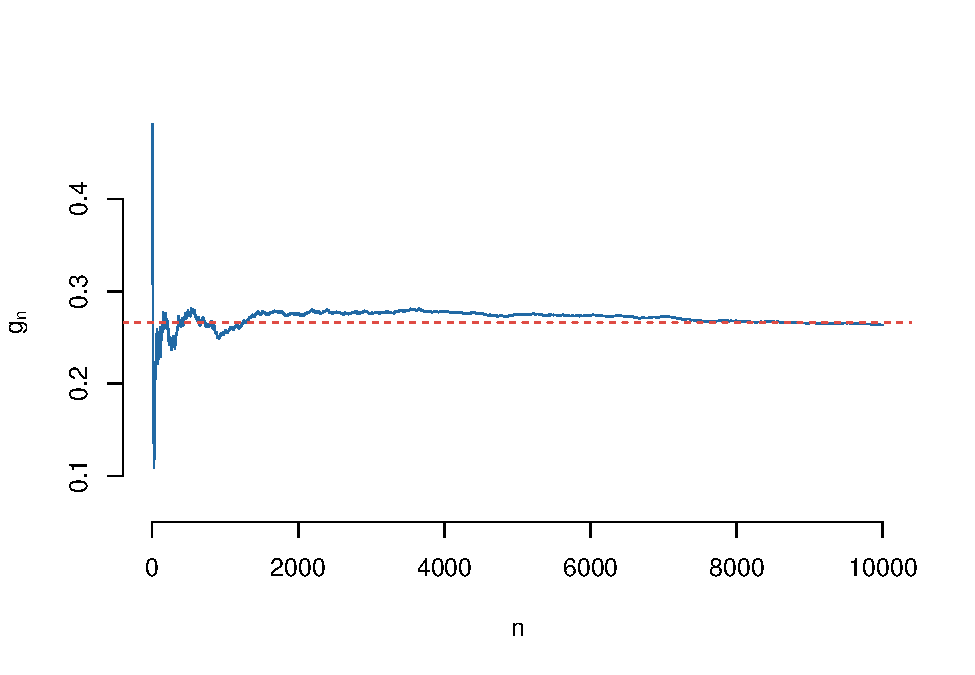
\includegraphics[width=0.8\linewidth]{Lab_2_files/figure-latex/unnamed-chunk-15-1} \end{center}

Observăm că probabilitatea de acoperire în acest caz este mai aproape de
ținta de \(1-\alpha = 0.95\) comparativ cu exemplul anterior.

\section{Testarea ipotezelor statistice: inferență asupra unui
eșantion}\label{testarea-ipotezelor-statistice-inferenta-asupra-unui-esantion}

\subsection{Exemplul 1}\label{exemplul-1}

\begin{rmdexercise}
Care este temperatura normală a corpului uman ?
(\href{readings/BodyTemp.pdf}{vezi articol}) Ne dorim să testăm din
punct de vedere statistic dacă temperatura medie a corpului uman este de
\(37^\circ C\) plecând de la următorul set de date
\href{dataIn/normtemp.txt}{descarcă} (sursa originală a datelor este
\emph{Mackowiak, P. A., Wasserman, S. S., and Levine, M. M. (1992). A
Critical Appraisal of 98.6 Degrees F, the Upper Limit of the Normal Body
Temperature, and Other Legacies of Carl Reinhold August Wunderlich.
Journal of the American Medical Association, 268, 1578-1580}).
\end{rmdexercise}

Pentru a citi datele putem folosi două metode: sau să le citim direct
din pagina de internet (prin comanda \texttt{read.table})

\begin{Shaded}
\begin{Highlighting}[]
\NormalTok{file =}\StringTok{ "https://alexamarioarei.github.io/Teaching/Biostat web page/labs/dataIn/normtemp.txt"}
\end{Highlighting}
\end{Shaded}

sau descărcând local fișierul cu date și înlocuind adresa de internet
din \texttt{file} cu cea locală

\begin{Shaded}
\begin{Highlighting}[]
\NormalTok{file =}\StringTok{ "dataIn/normtemp.txt"}
\NormalTok{normtemp =}\StringTok{ }\KeywordTok{read.table}\NormalTok{(file, }\DataTypeTok{header=}\NormalTok{F, }\DataTypeTok{col.names=}\KeywordTok{c}\NormalTok{(}\StringTok{"temp"}\NormalTok{,}\StringTok{"sex"}\NormalTok{,}\StringTok{"hr"}\NormalTok{))}

\KeywordTok{head}\NormalTok{(normtemp)}
\NormalTok{  temp sex hr}
\DecValTok{1} \FloatTok{96.3}   \DecValTok{1} \DecValTok{70}
\DecValTok{2} \FloatTok{96.7}   \DecValTok{1} \DecValTok{71}
\DecValTok{3} \FloatTok{96.9}   \DecValTok{1} \DecValTok{74}
\DecValTok{4} \FloatTok{97.0}   \DecValTok{1} \DecValTok{80}
\DecValTok{5} \FloatTok{97.1}   \DecValTok{1} \DecValTok{73}
\DecValTok{6} \FloatTok{97.1}   \DecValTok{1} \DecValTok{75}
\end{Highlighting}
\end{Shaded}

Temperatura apare în grade Fahrenheit și am dori să transformăm în grade
Celsius folosind formula:

\[
  T_C = 5(T_F-32)/9
\]

\begin{Shaded}
\begin{Highlighting}[]
\NormalTok{normtemp}\OperatorTok{$}\NormalTok{tempC =}\StringTok{ }\NormalTok{(normtemp}\OperatorTok{$}\NormalTok{temp }\OperatorTok{-}\StringTok{ }\DecValTok{32}\NormalTok{)}\OperatorTok{*}\DecValTok{5}\OperatorTok{/}\DecValTok{9} 
\NormalTok{degreesC =}\StringTok{ }\NormalTok{normtemp}\OperatorTok{$}\NormalTok{tempC}
\end{Highlighting}
\end{Shaded}

Testul t-student presupune că eșantionul (independent) a provenit
dintr-o populație normală și pentru aceasta putem verifica ipoteza de
normalitate (\texttt{QQ\ plot}):

\begin{Shaded}
\begin{Highlighting}[]
\KeywordTok{qqnorm}\NormalTok{(degreesC)}
\KeywordTok{qqline}\NormalTok{(degreesC)}
\end{Highlighting}
\end{Shaded}

\begin{center}\includegraphics[width=0.9\linewidth]{Lab_2_files/figure-latex/unnamed-chunk-20-1} \end{center}

Trasăm histograma:

\begin{Shaded}
\begin{Highlighting}[]
\KeywordTok{hist}\NormalTok{(degreesC, }\DataTypeTok{probability =}\NormalTok{ T)}
\NormalTok{degM =}\StringTok{ }\KeywordTok{mean}\NormalTok{(degreesC)}
\NormalTok{degSD =}\StringTok{ }\KeywordTok{sd}\NormalTok{(degreesC)}
\KeywordTok{curve}\NormalTok{(}\KeywordTok{dnorm}\NormalTok{(x, degM, degSD), }\DataTypeTok{add =}\NormalTok{ T, }\DataTypeTok{col =} \StringTok{"brown3"}\NormalTok{)}
\end{Highlighting}
\end{Shaded}

\begin{center}\includegraphics[width=0.9\linewidth]{Lab_2_files/figure-latex/unnamed-chunk-21-1} \end{center}

Trasăm densitatea:

\begin{Shaded}
\begin{Highlighting}[]
\KeywordTok{plot}\NormalTok{(}\KeywordTok{density}\NormalTok{(degreesC))}
\KeywordTok{curve}\NormalTok{(}\KeywordTok{dnorm}\NormalTok{(x, degM, degSD), }\DataTypeTok{add =}\NormalTok{ T, }\DataTypeTok{col =} \StringTok{"brown3"}\NormalTok{)}
\end{Highlighting}
\end{Shaded}

\begin{center}\includegraphics[width=0.9\linewidth]{Lab_2_files/figure-latex/unnamed-chunk-22-1} \end{center}

Testăm ipoteza de normalitate (folosind testul \texttt{Shapiro-Wilk}):

\begin{Shaded}
\begin{Highlighting}[]
\KeywordTok{shapiro.test}\NormalTok{(degreesC)}\CommentTok{# distributia pare sa fie aproape de normala si testul nu detecteaza }

\NormalTok{    Shapiro}\OperatorTok{-}\NormalTok{Wilk normality test}

\NormalTok{data}\OperatorTok{:}\StringTok{  }\NormalTok{degreesC}
\NormalTok{W =}\StringTok{ }\FloatTok{0.98658}\NormalTok{, p}\OperatorTok{-}\NormalTok{value =}\StringTok{ }\FloatTok{0.2332}
                      \CommentTok{# o abatere semnificativa fata de normala}
\end{Highlighting}
\end{Shaded}

Distribuția pare să fie aproape de normală, testul Shapiro-Wilk nu
detectează o deviație semnificantă de la normalitate.

\begin{Shaded}
\begin{Highlighting}[]
\KeywordTok{t.test}\NormalTok{(degreesC, }\DataTypeTok{mu =} \DecValTok{37}\NormalTok{, }\DataTypeTok{alternative =} \StringTok{"two.sided"}\NormalTok{) }\CommentTok{# respingem H0}

\NormalTok{    One Sample t}\OperatorTok{-}\NormalTok{test}

\NormalTok{data}\OperatorTok{:}\StringTok{  }\NormalTok{degreesC}
\NormalTok{t =}\StringTok{ }\OperatorTok{-}\FloatTok{5.4548}\NormalTok{, df =}\StringTok{ }\DecValTok{129}\NormalTok{, p}\OperatorTok{-}\NormalTok{value =}\StringTok{ }\FloatTok{2.411e-07}
\NormalTok{alternative hypothesis}\OperatorTok{:}\StringTok{ }\NormalTok{true mean is not equal to }\DecValTok{37}
\DecValTok{95}\NormalTok{ percent confidence interval}\OperatorTok{:}
\StringTok{ }\FloatTok{36.73445} \FloatTok{36.87581}
\NormalTok{sample estimates}\OperatorTok{:}
\NormalTok{mean of x }
 \FloatTok{36.80513} 
\end{Highlighting}
\end{Shaded}

\begin{Shaded}
\begin{Highlighting}[]
\NormalTok{ttest_deg =}\StringTok{ }\KeywordTok{t.test}\NormalTok{(degreesC, }\DataTypeTok{mu =} \DecValTok{37}\NormalTok{)}

\NormalTok{ttest_deg}\OperatorTok{$}\NormalTok{statistic}
\NormalTok{        t }
\OperatorTok{-}\FloatTok{5.454823} 
\NormalTok{ttest_deg}\OperatorTok{$}\NormalTok{p.value}
\NormalTok{[}\DecValTok{1}\NormalTok{] }\FloatTok{2.410632e-07}
\NormalTok{ttest_deg}\OperatorTok{$}\NormalTok{conf.int}
\NormalTok{[}\DecValTok{1}\NormalTok{] }\FloatTok{36.73445} \FloatTok{36.87581}
\KeywordTok{attr}\NormalTok{(,}\StringTok{"conf.level"}\NormalTok{)}
\NormalTok{[}\DecValTok{1}\NormalTok{] }\FloatTok{0.95}
\end{Highlighting}
\end{Shaded}

Dacă nu avem datele și avem o problemă de tipul: un eșantion de 130 de
persoane a fost selectionat și temperatura corpului a fost masurată.
Media eșantionului a fost \texttt{36.805} iar abaterea standard
\texttt{0.4073}. Testati ipoteza nulă că media temperaturii corpului
uman este de \texttt{37} grade Celsius.

În acest caz avem:

\begin{Shaded}
\begin{Highlighting}[]
\NormalTok{t.obt =}\StringTok{ }\NormalTok{(}\FloatTok{36.805} \OperatorTok{-}\StringTok{ }\DecValTok{37}\NormalTok{)}\OperatorTok{/}\NormalTok{(}\FloatTok{0.4073}\OperatorTok{/}\KeywordTok{sqrt}\NormalTok{(}\DecValTok{130}\NormalTok{))}
\NormalTok{t.obt}
\NormalTok{[}\DecValTok{1}\NormalTok{] }\OperatorTok{-}\FloatTok{5.458733}

\KeywordTok{qt}\NormalTok{(}\KeywordTok{c}\NormalTok{(}\FloatTok{0.25}\NormalTok{, }\FloatTok{0.975}\NormalTok{), }\DataTypeTok{df =} \DecValTok{129}\NormalTok{) }\CommentTok{# valorile critice pentru alpha = 0.05}
\NormalTok{[}\DecValTok{1}\NormalTok{] }\OperatorTok{-}\FloatTok{0.6763963}  \FloatTok{1.9785245}
\DecValTok{2}\OperatorTok{*}\KeywordTok{pt}\NormalTok{(t.obt, }\DataTypeTok{df =} \DecValTok{129}\NormalTok{) }\CommentTok{# p valoarea pentru testul two-tailed}
\NormalTok{[}\DecValTok{1}\NormalTok{] }\FloatTok{2.367923e-07}
\end{Highlighting}
\end{Shaded}

Ca să automatizăm aceste calcule putem crea o funcție:

\begin{Shaded}
\begin{Highlighting}[]
\NormalTok{t.single =}\StringTok{ }\ControlFlowTok{function}\NormalTok{(obs.mean, mu, SD, n) \{}
\NormalTok{  t.obt =}\StringTok{ }\NormalTok{(obs.mean }\OperatorTok{-}\StringTok{ }\NormalTok{mu) }\OperatorTok{/}\StringTok{ }\NormalTok{(SD }\OperatorTok{/}\StringTok{ }\KeywordTok{sqrt}\NormalTok{(n))}
\NormalTok{  p.value =}\StringTok{ }\KeywordTok{pt}\NormalTok{(}\KeywordTok{abs}\NormalTok{(t.obt), }\DataTypeTok{df=}\NormalTok{n}\OperatorTok{-}\DecValTok{1}\NormalTok{, }\DataTypeTok{lower.tail=}\NormalTok{F)}
  \KeywordTok{print}\NormalTok{(}\KeywordTok{c}\NormalTok{(}\DataTypeTok{t.obt =}\NormalTok{ t.obt, }\DataTypeTok{p.value =}\NormalTok{ p.value))}
  \KeywordTok{warning}\NormalTok{(}\StringTok{"P-value pentru one-sided. Dubleaza pentru two-sided."}\NormalTok{)}
\NormalTok{\}}

\KeywordTok{t.single}\NormalTok{(}\FloatTok{36.805}\NormalTok{, }\DataTypeTok{mu =} \DecValTok{37}\NormalTok{, }\DataTypeTok{SD =} \FloatTok{0.4073}\NormalTok{, }\DataTypeTok{n =} \DecValTok{130}\NormalTok{)}
\NormalTok{        t.obt       p.value }
\OperatorTok{-}\FloatTok{5.458733e+00}  \FloatTok{1.183961e-07} 
\NormalTok{Warning }\ControlFlowTok{in} \KeywordTok{t.single}\NormalTok{(}\FloatTok{36.805}\NormalTok{, }\DataTypeTok{mu =} \DecValTok{37}\NormalTok{, }\DataTypeTok{SD =} \FloatTok{0.4073}\NormalTok{, }\DataTypeTok{n =} \DecValTok{130}\NormalTok{)}\OperatorTok{:}\StringTok{ }\NormalTok{P}\OperatorTok{-}\NormalTok{value pentru}
\NormalTok{one}\OperatorTok{-}\NormalTok{sided. Dubleaza pentru two}\OperatorTok{-}\NormalTok{sided.}
\end{Highlighting}
\end{Shaded}

\section{Testarea ipotezelor statistice: inferență asupra a două
eșantioane}\label{testarea-ipotezelor-statistice-inferenta-asupra-a-doua-esantioane}

\subsection{Exemplul 1}\label{exemplul-1-1}

În contextul exemplului anterior, să presupunem că vrem să vedem dacă
există vreo diferență între temperatura medie la bărbați și temperatura
medie la femei.

\begin{Shaded}
\begin{Highlighting}[]
\KeywordTok{str}\NormalTok{(normtemp)}
\StringTok{'data.frame'}\OperatorTok{:}\StringTok{   }\DecValTok{130}\NormalTok{ obs. of  }\DecValTok{4}\NormalTok{ variables}\OperatorTok{:}
\StringTok{ }\ErrorTok{$}\StringTok{ }\NormalTok{temp }\OperatorTok{:}\StringTok{ }\NormalTok{num  }\FloatTok{96.3} \FloatTok{96.7} \FloatTok{96.9} \DecValTok{97} \FloatTok{97.1} \FloatTok{97.1} \FloatTok{97.1} \FloatTok{97.2} \FloatTok{97.3} \FloatTok{97.4}\NormalTok{ ...}
 \OperatorTok{$}\StringTok{ }\NormalTok{sex  }\OperatorTok{:}\StringTok{ }\NormalTok{int  }\DecValTok{1} \DecValTok{1} \DecValTok{1} \DecValTok{1} \DecValTok{1} \DecValTok{1} \DecValTok{1} \DecValTok{1} \DecValTok{1} \DecValTok{1}\NormalTok{ ...}
 \OperatorTok{$}\StringTok{ }\NormalTok{hr   }\OperatorTok{:}\StringTok{ }\NormalTok{int  }\DecValTok{70} \DecValTok{71} \DecValTok{74} \DecValTok{80} \DecValTok{73} \DecValTok{75} \DecValTok{82} \DecValTok{64} \DecValTok{69} \DecValTok{70}\NormalTok{ ...}
 \OperatorTok{$}\StringTok{ }\NormalTok{tempC}\OperatorTok{:}\StringTok{ }\NormalTok{num  }\FloatTok{35.7} \FloatTok{35.9} \FloatTok{36.1} \FloatTok{36.1} \FloatTok{36.2}\NormalTok{ ...}

\NormalTok{tempB =}\StringTok{ }\NormalTok{normtemp}\OperatorTok{$}\NormalTok{tempC[}\KeywordTok{which}\NormalTok{(normtemp}\OperatorTok{$}\NormalTok{sex }\OperatorTok{==}\StringTok{ }\DecValTok{1}\NormalTok{)]}
\NormalTok{tempF =}\StringTok{ }\NormalTok{normtemp}\OperatorTok{$}\NormalTok{tempC[}\KeywordTok{which}\NormalTok{(normtemp}\OperatorTok{$}\NormalTok{sex }\OperatorTok{==}\StringTok{ }\DecValTok{2}\NormalTok{)]}
\end{Highlighting}
\end{Shaded}

Ilustrare a temperaturii bărbaților și a femeilor:

\begin{Shaded}
\begin{Highlighting}[]
\KeywordTok{par}\NormalTok{(}\DataTypeTok{mfrow=}\KeywordTok{c}\NormalTok{(}\DecValTok{1}\NormalTok{,}\DecValTok{2}\NormalTok{))}
\KeywordTok{plot}\NormalTok{(}\KeywordTok{density}\NormalTok{(tempB), }\DataTypeTok{main=}\StringTok{"Temperatura Barbatilor"}\NormalTok{)}
\KeywordTok{plot}\NormalTok{(}\KeywordTok{density}\NormalTok{(tempF), }\DataTypeTok{main=}\StringTok{"Temperatura Femeilor"}\NormalTok{)}
\end{Highlighting}
\end{Shaded}

\begin{center}\includegraphics[width=0.9\linewidth]{Lab_2_files/figure-latex/unnamed-chunk-29-1} \end{center}

Sub formă de \texttt{boxplot}:

\begin{Shaded}
\begin{Highlighting}[]
\KeywordTok{par}\NormalTok{(}\DataTypeTok{mfrow =} \KeywordTok{c}\NormalTok{(}\DecValTok{1}\NormalTok{,}\DecValTok{1}\NormalTok{))}
\KeywordTok{boxplot}\NormalTok{(tempB, tempF, }\DataTypeTok{ylab=}\StringTok{"Temperatura"}\NormalTok{,     }\CommentTok{# plot and label y-axis}
                \DataTypeTok{names=}\KeywordTok{c}\NormalTok{(}\StringTok{"Barbati"}\NormalTok{,}\StringTok{"Femei"}\NormalTok{),   }\CommentTok{# group names on x-axis}
                \DataTypeTok{main=}\StringTok{"Temperatura in functie de sex"}\NormalTok{)   }\CommentTok{# main title}
\end{Highlighting}
\end{Shaded}

\begin{center}\includegraphics[width=0.9\linewidth]{Lab_2_files/figure-latex/unnamed-chunk-30-1} \end{center}

Trasarea datelor împreună cu intervalele de încredere:

\begin{Shaded}
\begin{Highlighting}[]
\KeywordTok{source}\NormalTok{(}\StringTok{"lab_functions/dotplot.R"}\NormalTok{)}

\KeywordTok{dotplot}\NormalTok{(tempB, tempF, }\DataTypeTok{labels=}\KeywordTok{c}\NormalTok{(}\StringTok{"Barbati"}\NormalTok{,}\StringTok{"Femei"}\NormalTok{))}
\end{Highlighting}
\end{Shaded}

\begin{center}\includegraphics[width=0.9\linewidth]{Lab_2_files/figure-latex/unnamed-chunk-31-1} \end{center}

Testarea ipotezelor statistice cu ajutorul testului t-student (corecția
lui \texttt{Welch}):

\begin{Shaded}
\begin{Highlighting}[]
\KeywordTok{t.test}\NormalTok{(tempB, tempF) }\CommentTok{# Welch correction }

\NormalTok{    Welch Two Sample t}\OperatorTok{-}\NormalTok{test}

\NormalTok{data}\OperatorTok{:}\StringTok{  }\NormalTok{tempB and tempF}
\NormalTok{t =}\StringTok{ }\OperatorTok{-}\FloatTok{2.2854}\NormalTok{, df =}\StringTok{ }\FloatTok{127.51}\NormalTok{, p}\OperatorTok{-}\NormalTok{value =}\StringTok{ }\FloatTok{0.02394}
\NormalTok{alternative hypothesis}\OperatorTok{:}\StringTok{ }\NormalTok{true difference }\ControlFlowTok{in}\NormalTok{ means is not equal to }\DecValTok{0}
\DecValTok{95}\NormalTok{ percent confidence interval}\OperatorTok{:}
\StringTok{ }\OperatorTok{-}\FloatTok{0.29980476} \OperatorTok{-}\FloatTok{0.02156277}
\NormalTok{sample estimates}\OperatorTok{:}
\NormalTok{mean of x mean of y }
 \FloatTok{36.72479}  \FloatTok{36.88547} 
\end{Highlighting}
\end{Shaded}

Verificăm dacă cele două eșantioane au varianțe egale (folosim testul
lui \texttt{Fisher}):

\begin{Shaded}
\begin{Highlighting}[]
\KeywordTok{var.test}\NormalTok{(tempB, tempF)}

\NormalTok{    F test to compare two variances}

\NormalTok{data}\OperatorTok{:}\StringTok{  }\NormalTok{tempB and tempF}
\NormalTok{F =}\StringTok{ }\FloatTok{0.88329}\NormalTok{, num df =}\StringTok{ }\DecValTok{64}\NormalTok{, denom df =}\StringTok{ }\DecValTok{64}\NormalTok{, p}\OperatorTok{-}\NormalTok{value =}\StringTok{ }\FloatTok{0.6211}
\NormalTok{alternative hypothesis}\OperatorTok{:}\StringTok{ }\NormalTok{true ratio of variances is not equal to }\DecValTok{1}
\DecValTok{95}\NormalTok{ percent confidence interval}\OperatorTok{:}
\StringTok{ }\FloatTok{0.5387604} \FloatTok{1.4481404}
\NormalTok{sample estimates}\OperatorTok{:}
\NormalTok{ratio of variances }
         \FloatTok{0.8832897} 
\end{Highlighting}
\end{Shaded}

Aplicăm acum testul t-student cu opțiunea de varianțe egale
(\texttt{pooled\ variance}):

\begin{Shaded}
\begin{Highlighting}[]
\KeywordTok{t.test}\NormalTok{(tempB, tempF, }\DataTypeTok{var.equal =}\NormalTok{ T) }\CommentTok{# without Welch correction }

\NormalTok{    Two Sample t}\OperatorTok{-}\NormalTok{test}

\NormalTok{data}\OperatorTok{:}\StringTok{  }\NormalTok{tempB and tempF}
\NormalTok{t =}\StringTok{ }\OperatorTok{-}\FloatTok{2.2854}\NormalTok{, df =}\StringTok{ }\DecValTok{128}\NormalTok{, p}\OperatorTok{-}\NormalTok{value =}\StringTok{ }\FloatTok{0.02393}
\NormalTok{alternative hypothesis}\OperatorTok{:}\StringTok{ }\NormalTok{true difference }\ControlFlowTok{in}\NormalTok{ means is not equal to }\DecValTok{0}
\DecValTok{95}\NormalTok{ percent confidence interval}\OperatorTok{:}
\StringTok{ }\OperatorTok{-}\FloatTok{0.29979966} \OperatorTok{-}\FloatTok{0.02156786}
\NormalTok{sample estimates}\OperatorTok{:}
\NormalTok{mean of x mean of y }
 \FloatTok{36.72479}  \FloatTok{36.88547} 
\end{Highlighting}
\end{Shaded}

\subsection{Exemplul 2}\label{exemplul-2}

\begin{Shaded}
\begin{Highlighting}[]
\CommentTok{# Example data}
\NormalTok{x <-}\StringTok{ }\KeywordTok{c}\NormalTok{(}\FloatTok{102.5}\NormalTok{, }\FloatTok{106.6}\NormalTok{,  }\FloatTok{99.8}\NormalTok{, }\FloatTok{106.5}\NormalTok{, }\FloatTok{103.7}\NormalTok{, }\FloatTok{105.5}\NormalTok{, }\FloatTok{98.2}\NormalTok{, }\FloatTok{104.1}\NormalTok{,  }\FloatTok{85.6}\NormalTok{, }\FloatTok{105.5}\NormalTok{, }\FloatTok{114.0}\NormalTok{, }\FloatTok{112.2}\NormalTok{)}
\NormalTok{y <-}\StringTok{ }\KeywordTok{c}\NormalTok{( }\FloatTok{93.7}\NormalTok{,  }\FloatTok{90.9}\NormalTok{, }\FloatTok{100.4}\NormalTok{,  }\FloatTok{92.0}\NormalTok{, }\FloatTok{100.2}\NormalTok{, }\FloatTok{104.6}\NormalTok{, }\FloatTok{95.4}\NormalTok{,  }\FloatTok{96.6}\NormalTok{,  }\FloatTok{99.2}\NormalTok{)}

\CommentTok{# Two-sided t-test allowing un-equal population SDs}
\KeywordTok{t.test}\NormalTok{(x,y)}

\NormalTok{    Welch Two Sample t}\OperatorTok{-}\NormalTok{test}

\NormalTok{data}\OperatorTok{:}\StringTok{  }\NormalTok{x and y}
\NormalTok{t =}\StringTok{ }\FloatTok{2.6041}\NormalTok{, df =}\StringTok{ }\FloatTok{18.475}\NormalTok{, p}\OperatorTok{-}\NormalTok{value =}\StringTok{ }\FloatTok{0.01769}
\NormalTok{alternative hypothesis}\OperatorTok{:}\StringTok{ }\NormalTok{true difference }\ControlFlowTok{in}\NormalTok{ means is not equal to }\DecValTok{0}
\DecValTok{95}\NormalTok{ percent confidence interval}\OperatorTok{:}
\StringTok{  }\FloatTok{1.30124} \FloatTok{12.06543}
\NormalTok{sample estimates}\OperatorTok{:}
\NormalTok{mean of x mean of y }
 \FloatTok{103.6833}   \FloatTok{97.0000} 

\KeywordTok{dotplot}\NormalTok{(x,y)}
\end{Highlighting}
\end{Shaded}

\begin{center}\includegraphics[width=0.9\linewidth]{Lab_2_files/figure-latex/unnamed-chunk-35-1} \end{center}

\subsection{Exemplul 3}\label{exemplul-3}

\begin{Shaded}
\begin{Highlighting}[]
\CommentTok{# One-tailed test example}
\NormalTok{x <-}\StringTok{ }\KeywordTok{c}\NormalTok{(}\FloatTok{59.4}\NormalTok{, }\FloatTok{52.3}\NormalTok{, }\FloatTok{42.6}\NormalTok{, }\FloatTok{45.1}\NormalTok{, }\FloatTok{65.9}\NormalTok{, }\FloatTok{40.8}\NormalTok{)}
\NormalTok{y <-}\StringTok{ }\KeywordTok{c}\NormalTok{(}\FloatTok{82.7}\NormalTok{, }\FloatTok{56.7}\NormalTok{, }\FloatTok{46.9}\NormalTok{, }\FloatTok{67.8}\NormalTok{, }\FloatTok{74.8}\NormalTok{, }\FloatTok{85.7}\NormalTok{)}

\CommentTok{# One-tailed t-test}
\KeywordTok{t.test}\NormalTok{(x,y,}\DataTypeTok{alt=}\StringTok{"less"}\NormalTok{)}

\NormalTok{    Welch Two Sample t}\OperatorTok{-}\NormalTok{test}

\NormalTok{data}\OperatorTok{:}\StringTok{  }\NormalTok{x and y}
\NormalTok{t =}\StringTok{ }\OperatorTok{-}\FloatTok{2.4421}\NormalTok{, df =}\StringTok{ }\FloatTok{8.6937}\NormalTok{, p}\OperatorTok{-}\NormalTok{value =}\StringTok{ }\FloatTok{0.01907}
\NormalTok{alternative hypothesis}\OperatorTok{:}\StringTok{ }\NormalTok{true difference }\ControlFlowTok{in}\NormalTok{ means is less than }\DecValTok{0}
\DecValTok{95}\NormalTok{ percent confidence interval}\OperatorTok{:}
\StringTok{      }\OperatorTok{-}\OtherTok{Inf} \OperatorTok{-}\FloatTok{4.454703}
\NormalTok{sample estimates}\OperatorTok{:}
\NormalTok{mean of x mean of y }
 \FloatTok{51.01667}  \FloatTok{69.10000} 

\CommentTok{# The dotplot}
\KeywordTok{dotplot}\NormalTok{(x,y)}
\end{Highlighting}
\end{Shaded}

\begin{center}\includegraphics[width=0.9\linewidth]{Lab_2_files/figure-latex/unnamed-chunk-36-1} \end{center}

\subsection{Exemplul 4}\label{exemplul-4}

\begin{Shaded}
\begin{Highlighting}[]
\CommentTok{# another one-tailed test example}
\NormalTok{x <-}\StringTok{ }\KeywordTok{c}\NormalTok{(}\FloatTok{63.3}\NormalTok{, }\FloatTok{58.6}\NormalTok{, }\FloatTok{59.0}\NormalTok{, }\FloatTok{60.5}\NormalTok{, }\FloatTok{56.3}\NormalTok{, }\FloatTok{57.4}\NormalTok{)}
\NormalTok{y <-}\StringTok{ }\KeywordTok{c}\NormalTok{(}\FloatTok{75.6}\NormalTok{, }\FloatTok{65.9}\NormalTok{, }\FloatTok{72.3}\NormalTok{, }\FloatTok{58.0}\NormalTok{, }\FloatTok{64.4}\NormalTok{, }\FloatTok{66.2}\NormalTok{)}
\KeywordTok{t.test}\NormalTok{(x,y,}\DataTypeTok{alt=}\StringTok{"less"}\NormalTok{)}

\NormalTok{    Welch Two Sample t}\OperatorTok{-}\NormalTok{test}

\NormalTok{data}\OperatorTok{:}\StringTok{  }\NormalTok{x and y}
\NormalTok{t =}\StringTok{ }\OperatorTok{-}\FloatTok{2.8968}\NormalTok{, df =}\StringTok{ }\FloatTok{6.5546}\NormalTok{, p}\OperatorTok{-}\NormalTok{value =}\StringTok{ }\FloatTok{0.01242}
\NormalTok{alternative hypothesis}\OperatorTok{:}\StringTok{ }\NormalTok{true difference }\ControlFlowTok{in}\NormalTok{ means is less than }\DecValTok{0}
\DecValTok{95}\NormalTok{ percent confidence interval}\OperatorTok{:}
\StringTok{      }\OperatorTok{-}\OtherTok{Inf} \OperatorTok{-}\FloatTok{2.674212}
\NormalTok{sample estimates}\OperatorTok{:}
\NormalTok{mean of x mean of y }
 \FloatTok{59.18333}  \FloatTok{67.06667} 
\KeywordTok{dotplot}\NormalTok{(x,y)}
\end{Highlighting}
\end{Shaded}

\begin{center}\includegraphics[width=0.9\linewidth]{Lab_2_files/figure-latex/unnamed-chunk-37-1} \end{center}

\subsection{Un model de grafic}\label{un-model-de-grafic}

\begin{Shaded}
\begin{Highlighting}[]
\NormalTok{x <-}\StringTok{ }\KeywordTok{c}\NormalTok{(}\FloatTok{15.1}\NormalTok{, }\FloatTok{13.1}\NormalTok{, }\FloatTok{21.5}\NormalTok{)}
\NormalTok{y <-}\StringTok{ }\KeywordTok{c}\NormalTok{(}\FloatTok{35.1}\NormalTok{, }\FloatTok{39.5}\NormalTok{, }\FloatTok{58.8}\NormalTok{)}

\KeywordTok{par}\NormalTok{(}\DataTypeTok{mar=}\KeywordTok{c}\NormalTok{(}\DecValTok{4}\NormalTok{,}\DecValTok{4}\NormalTok{,}\DecValTok{2}\NormalTok{,}\DecValTok{1}\NormalTok{),}\DataTypeTok{mfrow=}\KeywordTok{c}\NormalTok{(}\DecValTok{1}\NormalTok{,}\DecValTok{2}\NormalTok{),}\DataTypeTok{las=}\DecValTok{1}\NormalTok{)}

\KeywordTok{barplot}\NormalTok{(}\KeywordTok{c}\NormalTok{(}\KeywordTok{mean}\NormalTok{(x),}\KeywordTok{mean}\NormalTok{(y)),}\DataTypeTok{width=}\DecValTok{1}\NormalTok{,}\DataTypeTok{space=}\KeywordTok{c}\NormalTok{(}\FloatTok{0.5}\NormalTok{,}\FloatTok{0.5}\NormalTok{),}
        \DataTypeTok{col=}\KeywordTok{c}\NormalTok{(}\StringTok{"white"}\NormalTok{,}\StringTok{"gray40"}\NormalTok{),}\DataTypeTok{xlim=}\KeywordTok{c}\NormalTok{(}\DecValTok{0}\NormalTok{,}\DecValTok{3}\NormalTok{),}\DataTypeTok{names=}\KeywordTok{c}\NormalTok{(}\StringTok{"A"}\NormalTok{,}\StringTok{"B"}\NormalTok{),}
        \DataTypeTok{ylim=}\KeywordTok{c}\NormalTok{(}\DecValTok{0}\NormalTok{,}\DecValTok{76}\NormalTok{))}
\KeywordTok{segments}\NormalTok{(}\DecValTok{1}\NormalTok{,}\KeywordTok{mean}\NormalTok{(x),}\DecValTok{1}\NormalTok{,}\KeywordTok{mean}\NormalTok{(x)}\OperatorTok{+}\KeywordTok{sd}\NormalTok{(x),}\DataTypeTok{lwd=}\DecValTok{2}\NormalTok{)}
\KeywordTok{segments}\NormalTok{(}\FloatTok{0.8}\NormalTok{,}\KeywordTok{mean}\NormalTok{(x)}\OperatorTok{+}\KeywordTok{sd}\NormalTok{(x),}\FloatTok{1.2}\NormalTok{,}\KeywordTok{mean}\NormalTok{(x)}\OperatorTok{+}\KeywordTok{sd}\NormalTok{(x),}\DataTypeTok{lwd=}\DecValTok{2}\NormalTok{)}
\KeywordTok{segments}\NormalTok{(}\FloatTok{2.5}\NormalTok{,}\KeywordTok{mean}\NormalTok{(y),}\FloatTok{2.5}\NormalTok{,}\KeywordTok{mean}\NormalTok{(y)}\OperatorTok{+}\KeywordTok{sd}\NormalTok{(y),}\DataTypeTok{lwd=}\DecValTok{2}\NormalTok{)}
\KeywordTok{segments}\NormalTok{(}\FloatTok{2.3}\NormalTok{,}\KeywordTok{mean}\NormalTok{(y)}\OperatorTok{+}\KeywordTok{sd}\NormalTok{(y),}\FloatTok{2.7}\NormalTok{,}\KeywordTok{mean}\NormalTok{(y)}\OperatorTok{+}\KeywordTok{sd}\NormalTok{(y),}\DataTypeTok{lwd=}\DecValTok{2}\NormalTok{)}
\KeywordTok{mtext}\NormalTok{(}\StringTok{"Grafic nepotrivit"}\NormalTok{,}\DataTypeTok{cex=}\FloatTok{1.5}\NormalTok{,}\DataTypeTok{line=}\FloatTok{0.5}\NormalTok{)}

\KeywordTok{plot}\NormalTok{(}\KeywordTok{rep}\NormalTok{(}\DecValTok{0}\OperatorTok{:}\DecValTok{1}\NormalTok{,}\KeywordTok{c}\NormalTok{(}\DecValTok{3}\NormalTok{,}\DecValTok{3}\NormalTok{)),}\KeywordTok{c}\NormalTok{(x,y),}\DataTypeTok{xaxt=}\StringTok{"n"}\NormalTok{,}\DataTypeTok{ylim=}\KeywordTok{c}\NormalTok{(}\DecValTok{0}\NormalTok{,}\DecValTok{76}\NormalTok{),}
     \DataTypeTok{xlim=}\KeywordTok{c}\NormalTok{(}\OperatorTok{-}\FloatTok{0.5}\NormalTok{,}\FloatTok{1.5}\NormalTok{),}\DataTypeTok{ylab=}\StringTok{""}\NormalTok{,}\DataTypeTok{xlab=}\StringTok{""}\NormalTok{)}
\KeywordTok{abline}\NormalTok{(}\DataTypeTok{v=}\DecValTok{0}\OperatorTok{:}\DecValTok{1}\NormalTok{,}\DataTypeTok{col=}\StringTok{"gray40"}\NormalTok{,}\DataTypeTok{lty=}\DecValTok{2}\NormalTok{)}
\KeywordTok{points}\NormalTok{(}\KeywordTok{rep}\NormalTok{(}\DecValTok{0}\OperatorTok{:}\DecValTok{1}\NormalTok{,}\KeywordTok{c}\NormalTok{(}\DecValTok{3}\NormalTok{,}\DecValTok{3}\NormalTok{)),}\KeywordTok{c}\NormalTok{(x,y),}\DataTypeTok{lwd=}\DecValTok{2}\NormalTok{)}
\KeywordTok{mtext}\NormalTok{(}\StringTok{"Grafic recomandat"}\NormalTok{,}\DataTypeTok{cex=}\FloatTok{1.5}\NormalTok{,}\DataTypeTok{line=}\FloatTok{0.5}\NormalTok{)}
\NormalTok{xci <-}\StringTok{ }\KeywordTok{t.test}\NormalTok{(x)}\OperatorTok{$}\NormalTok{conf.int}
\NormalTok{yci <-}\StringTok{ }\KeywordTok{t.test}\NormalTok{(y)}\OperatorTok{$}\NormalTok{conf.int}
\KeywordTok{segments}\NormalTok{(}\FloatTok{0.25}\NormalTok{,xci[}\DecValTok{1}\NormalTok{],}\FloatTok{0.25}\NormalTok{,xci[}\DecValTok{2}\NormalTok{],}\DataTypeTok{lwd=}\DecValTok{2}\NormalTok{,}\DataTypeTok{col=}\StringTok{"darkgray"}\NormalTok{)}
\KeywordTok{segments}\NormalTok{(}\KeywordTok{c}\NormalTok{(}\FloatTok{0.23}\NormalTok{,}\FloatTok{0.23}\NormalTok{,}\FloatTok{0.2}\NormalTok{),}\KeywordTok{c}\NormalTok{(xci,}\KeywordTok{mean}\NormalTok{(x)),}\KeywordTok{c}\NormalTok{(}\FloatTok{0.27}\NormalTok{,}\FloatTok{0.27}\NormalTok{,}\FloatTok{0.3}\NormalTok{),}
         \KeywordTok{c}\NormalTok{(xci,}\KeywordTok{mean}\NormalTok{(x)),}\DataTypeTok{lwd=}\DecValTok{2}\NormalTok{,}\DataTypeTok{col=}\StringTok{"darkgray"}\NormalTok{)}
\KeywordTok{segments}\NormalTok{(}\DecValTok{1}\OperatorTok{-}\FloatTok{0.25}\NormalTok{,yci[}\DecValTok{1}\NormalTok{],}\DecValTok{1}\OperatorTok{-}\FloatTok{0.25}\NormalTok{,yci[}\DecValTok{2}\NormalTok{],}\DataTypeTok{lwd=}\DecValTok{2}\NormalTok{,}\DataTypeTok{col=}\StringTok{"brown3"}\NormalTok{)}
\KeywordTok{segments}\NormalTok{(}\DecValTok{1}\OperatorTok{-}\KeywordTok{c}\NormalTok{(}\FloatTok{0.23}\NormalTok{,}\FloatTok{0.23}\NormalTok{,}\FloatTok{0.2}\NormalTok{),}\KeywordTok{c}\NormalTok{(yci,}\KeywordTok{mean}\NormalTok{(y)),}\DecValTok{1}\OperatorTok{-}\KeywordTok{c}\NormalTok{(}\FloatTok{0.27}\NormalTok{,}\FloatTok{0.27}\NormalTok{,}\FloatTok{0.3}\NormalTok{),}
         \KeywordTok{c}\NormalTok{(yci,}\KeywordTok{mean}\NormalTok{(y)),}\DataTypeTok{lwd=}\DecValTok{2}\NormalTok{,}\DataTypeTok{col=}\StringTok{"brown3"}\NormalTok{)}
\NormalTok{u <-}\StringTok{ }\KeywordTok{par}\NormalTok{(}\StringTok{"usr"}\NormalTok{)}
\KeywordTok{segments}\NormalTok{(}\DecValTok{0}\OperatorTok{:}\DecValTok{1}\NormalTok{,u[}\DecValTok{3}\NormalTok{],}\DecValTok{0}\OperatorTok{:}\DecValTok{1}\NormalTok{,u[}\DecValTok{3}\NormalTok{]}\OperatorTok{-}\KeywordTok{diff}\NormalTok{(u[}\DecValTok{3}\OperatorTok{:}\DecValTok{4}\NormalTok{])}\OperatorTok{*}\FloatTok{0.03}\NormalTok{,}\DataTypeTok{xpd=}\OtherTok{TRUE}\NormalTok{)}
\KeywordTok{text}\NormalTok{(}\DecValTok{0}\OperatorTok{:}\DecValTok{1}\NormalTok{,u[}\DecValTok{3}\NormalTok{]}\OperatorTok{-}\KeywordTok{diff}\NormalTok{(u[}\DecValTok{3}\OperatorTok{:}\DecValTok{4}\NormalTok{])}\OperatorTok{*}\FloatTok{0.08}\NormalTok{,}\KeywordTok{c}\NormalTok{(}\StringTok{"A"}\NormalTok{,}\StringTok{"B"}\NormalTok{),}\DataTypeTok{xpd=}\OtherTok{TRUE}\NormalTok{)}
\end{Highlighting}
\end{Shaded}

\begin{center}\includegraphics[width=0.9\linewidth]{Lab_2_files/figure-latex/unnamed-chunk-38-1} \end{center}

\section{Testarea ipotezelor statistice: inferență asupra a două
eșantioane dependente
(perechi)}\label{testarea-ipotezelor-statistice-inferenta-asupra-a-doua-esantioane-dependente-perechi}

Considerăm următorul set de date din pachetul \texttt{MASS} (luarea in
greutate de catre femei anorexice):

\begin{Shaded}
\begin{Highlighting}[]
\KeywordTok{data}\NormalTok{(anorexia, }\DataTypeTok{package=}\StringTok{"MASS"}\NormalTok{)      }
\KeywordTok{attach}\NormalTok{(anorexia)}
\KeywordTok{str}\NormalTok{(anorexia)}
\StringTok{'data.frame'}\OperatorTok{:}\StringTok{   }\DecValTok{72}\NormalTok{ obs. of  }\DecValTok{3}\NormalTok{ variables}\OperatorTok{:}
\StringTok{ }\ErrorTok{$}\StringTok{ }\NormalTok{Treat }\OperatorTok{:}\StringTok{ }\NormalTok{Factor w}\OperatorTok{/}\StringTok{ }\DecValTok{3}\NormalTok{ levels }\StringTok{"CBT"}\NormalTok{,}\StringTok{"Cont"}\NormalTok{,}\StringTok{"FT"}\OperatorTok{:}\StringTok{ }\DecValTok{2} \DecValTok{2} \DecValTok{2} \DecValTok{2} \DecValTok{2} \DecValTok{2} \DecValTok{2} \DecValTok{2} \DecValTok{2} \DecValTok{2}\NormalTok{ ...}
 \OperatorTok{$}\StringTok{ }\NormalTok{Prewt }\OperatorTok{:}\StringTok{ }\NormalTok{num  }\FloatTok{80.7} \FloatTok{89.4} \FloatTok{91.8} \DecValTok{74} \FloatTok{78.1} \FloatTok{88.3} \FloatTok{87.3} \FloatTok{75.1} \FloatTok{80.6} \FloatTok{78.4}\NormalTok{ ...}
 \OperatorTok{$}\StringTok{ }\NormalTok{Postwt}\OperatorTok{:}\StringTok{ }\NormalTok{num  }\FloatTok{80.2} \FloatTok{80.1} \FloatTok{86.4} \FloatTok{86.3} \FloatTok{76.1} \FloatTok{78.1} \FloatTok{75.1} \FloatTok{86.7} \FloatTok{73.5} \FloatTok{84.6}\NormalTok{ ...}

\NormalTok{ft=}\KeywordTok{subset}\NormalTok{(anorexia,}\DataTypeTok{Treat=}\StringTok{"FT"}\NormalTok{) }\CommentTok{# family treatment}
\end{Highlighting}
\end{Shaded}

Testăm dacă există diferențe între luarea în greutate înainte de
tratament și după tratament:

\begin{Shaded}
\begin{Highlighting}[]
\KeywordTok{with}\NormalTok{(ft, }\KeywordTok{t.test}\NormalTok{(Postwt}\OperatorTok{-}\NormalTok{Prewt, }\DataTypeTok{mu=}\DecValTok{0}\NormalTok{, }\DataTypeTok{alternative=}\StringTok{"greater"}\NormalTok{))}

\NormalTok{    One Sample t}\OperatorTok{-}\NormalTok{test}

\NormalTok{data}\OperatorTok{:}\StringTok{  }\NormalTok{Postwt }\OperatorTok{-}\StringTok{ }\NormalTok{Prewt}
\NormalTok{t =}\StringTok{ }\FloatTok{2.9376}\NormalTok{, df =}\StringTok{ }\DecValTok{71}\NormalTok{, p}\OperatorTok{-}\NormalTok{value =}\StringTok{ }\FloatTok{0.002229}
\NormalTok{alternative hypothesis}\OperatorTok{:}\StringTok{ }\NormalTok{true mean is greater than }\DecValTok{0}
\DecValTok{95}\NormalTok{ percent confidence interval}\OperatorTok{:}
\StringTok{ }\FloatTok{1.195825}      \OtherTok{Inf}
\NormalTok{sample estimates}\OperatorTok{:}
\NormalTok{mean of x }
 \FloatTok{2.763889} 
\end{Highlighting}
\end{Shaded}

sau

\begin{Shaded}
\begin{Highlighting}[]
\KeywordTok{with}\NormalTok{(ft, }\KeywordTok{t.test}\NormalTok{(Postwt, Prewt, }\DataTypeTok{paired=}\NormalTok{T, }\DataTypeTok{alternative=}\StringTok{"greater"}\NormalTok{))}

\NormalTok{    Paired t}\OperatorTok{-}\NormalTok{test}

\NormalTok{data}\OperatorTok{:}\StringTok{  }\NormalTok{Postwt and Prewt}
\NormalTok{t =}\StringTok{ }\FloatTok{2.9376}\NormalTok{, df =}\StringTok{ }\DecValTok{71}\NormalTok{, p}\OperatorTok{-}\NormalTok{value =}\StringTok{ }\FloatTok{0.002229}
\NormalTok{alternative hypothesis}\OperatorTok{:}\StringTok{ }\NormalTok{true difference }\ControlFlowTok{in}\NormalTok{ means is greater than }\DecValTok{0}
\DecValTok{95}\NormalTok{ percent confidence interval}\OperatorTok{:}
\StringTok{ }\FloatTok{1.195825}      \OtherTok{Inf}
\NormalTok{sample estimates}\OperatorTok{:}
\NormalTok{mean of the differences }
               \FloatTok{2.763889} 
\end{Highlighting}
\end{Shaded}


\end{document}
